% !TeX spellcheck = en_GB
% !TeX spellcheck = en_US 

\chapter{Results and Discussion}

As mentioned, this experiment was performed in two laser facilities. At The Extreme light Infrastructure beamlines ELI-ALPS in Szeged, Hungary, and at the Max Plank institute for nuclear physics in Heidelberg, Germany. In this chapter we will present the results of different experiments in an individual way, finalizing with a comparison of HE cluster in the two different laser fields (MIR and NIR) and Ne and He at the MIR laser. As above, all data were selected and treated as single nanoplasma explosions signals, with independent calibrations.

In the first part of the chapter we will present the results for Helium cluster under NIR field. The Experiment was done in Heidelberg with a Ti-Sr $800nm$ wavelength laser. An intensity scan, Droplet size dependence and Xe doping dependence are introduced. The second section will show the results of Helium clusters under a $3200$ nm wavelength (MIR) in Szeged, where we make measurements  of  cluster size dependence, Xe-Ca doping scans, Ar doping scan,  water doping scan and pulse duration scan. Finally we present the results at the second beam time in ELI, similar experiments were performed with the same laser but with Neon as cluster source. Measurements of Cluster size dependence, Pulse duration Scan and Xe doping scan were also performed. For additional information about the laser system used in each of the Beam lines, we recommended to the reader to find the detailed characteristics in the next links, \cite {thire_highly_2018}.


Fig. \ref{fig:rawMIRHESIZE} shows an example of some background subtracted electron-VMI raw signal. From now on, we will refer electron-VMI just as VMI. On fig. \ref{fig:rawMIRHESIZE} d. shows one of the outline founded in the bigger explosion  where the He signal presents few electrons with low energy, given it a ring shape that we will denominate "Donut" shape. The helium and neon signals present quite similarities, except for the donut shape. The signal radius along a data set changes constantly and each individual signal need to be analyzed independently. In general parameters as the voltage in the system and the wear and tear of the detector also needs to be taken into account. Non Abel transform is necessary because we will deal with the maximum energy distribution only, and just to detect the radius in the signal is suitable. The distribution of radius and brightness in the images will be translated to an Energy-Numb Electrons distribution, in order to get some information about the density and reachable energy in the coulomb explosion, as show in the next sections.

\begin{figure}[h!]
\centering
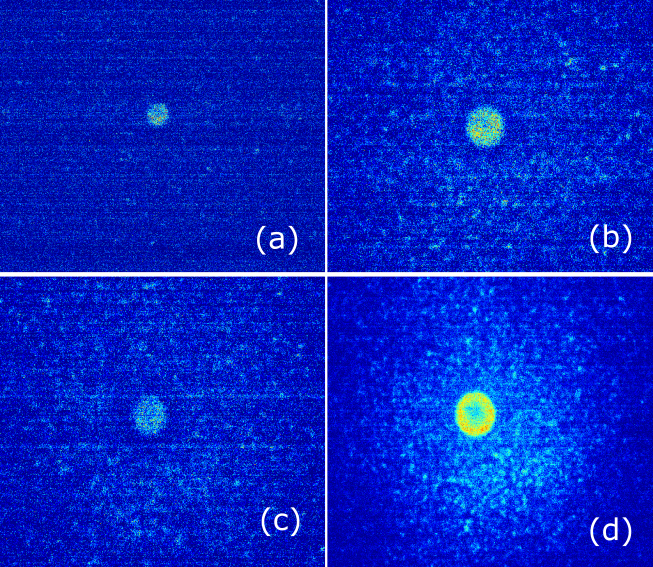
\includegraphics[width =12 cm]{../Images/results/Mir_He_Dropletsize/rawimageSample.png}
\caption[He-Xe dop, raw image]{Example raw images of VMI for the droplet size scan from one data set. Images a, b and c present different size and intensities but a uniform circular shape while figure d, presents a "donut" shape.}
\label{fig:rawMIRHESIZE}
\end{figure}

\section{Helium nanoplasma under NIR Fields}

As presented on the experimental setup, we can modify several parameters to perform different experiments in order to understand better the nanoplasma process. The cluster can be created, at different nozzle temperatures, given different droplet sizes. He can be doped with one or two dopant at different densities varying the pressures of the dopant gas or the temperature of the oven. Finally the cluster will be ignited in a coulomb explosion due the femtosecond laser pulse and the electrons will be detected by the VMI and the Ions will be detected by the TOF. 

In the next sections, special attention will be taken on the VMI results due the amount of information it can deliver. The TOF data, is analyzed in an independent way, but will not be part of the main results. The data done in Heidelberg were already analyzed in the master thesis of Nicolas Rendler and the information can be found in \cite{rendler_einzelschuss_2017}. The main purpose to re-evaluate this information is to compare the experiments with similar parameters to the ones used in ELI-AlPS.

Using the "Xenon ion charge" intensity calibration, on the NIR laser they obtained table \ref{tab:nirintens}with the corresponding to the focused intensities depending on the power. The laser power was measured just before the beam enters to the detection chamber and was compared also to the theoretical calculations for the optical system mounted as shown in Fig. \ref{fig:xeionchargecalib}. As we could observe, the signal rate in each data set depends on the intensity at the focus, for the nano plasma a minimum field energy is needed to start the ionization on the dopant and hence, start the coulomb explosion. In order to have the best results and high data acquisition, we worked at maximum intensity near $55mW$, so we can ensure the good quality of the ignition process and hence its efficiency.

\begin{table}[t]

\centering
\begin{tabular}{|l|c|}
\hline
\multicolumn{1}{|c|}{$Power{[}mW{]}$} & $Laser intensity {[}W/Cm^{2}{]}$ \\ \hline
11                                  & 6,27E13                                           \\ \hline
25                                  & 1,425E14                                          \\ \hline
55                                  & 3,135E14                                          \\ \hline
80                                  & 4,56E14                                           \\ \hline
115                                 & 6,555E14                                          \\ \hline
\end{tabular}
\caption[NIR laser power to intensities]{Laser focused intensities calculated for different Powers }
\label{tab:nirintens}
\end{table}


\begin{figure}[h!]
\centering
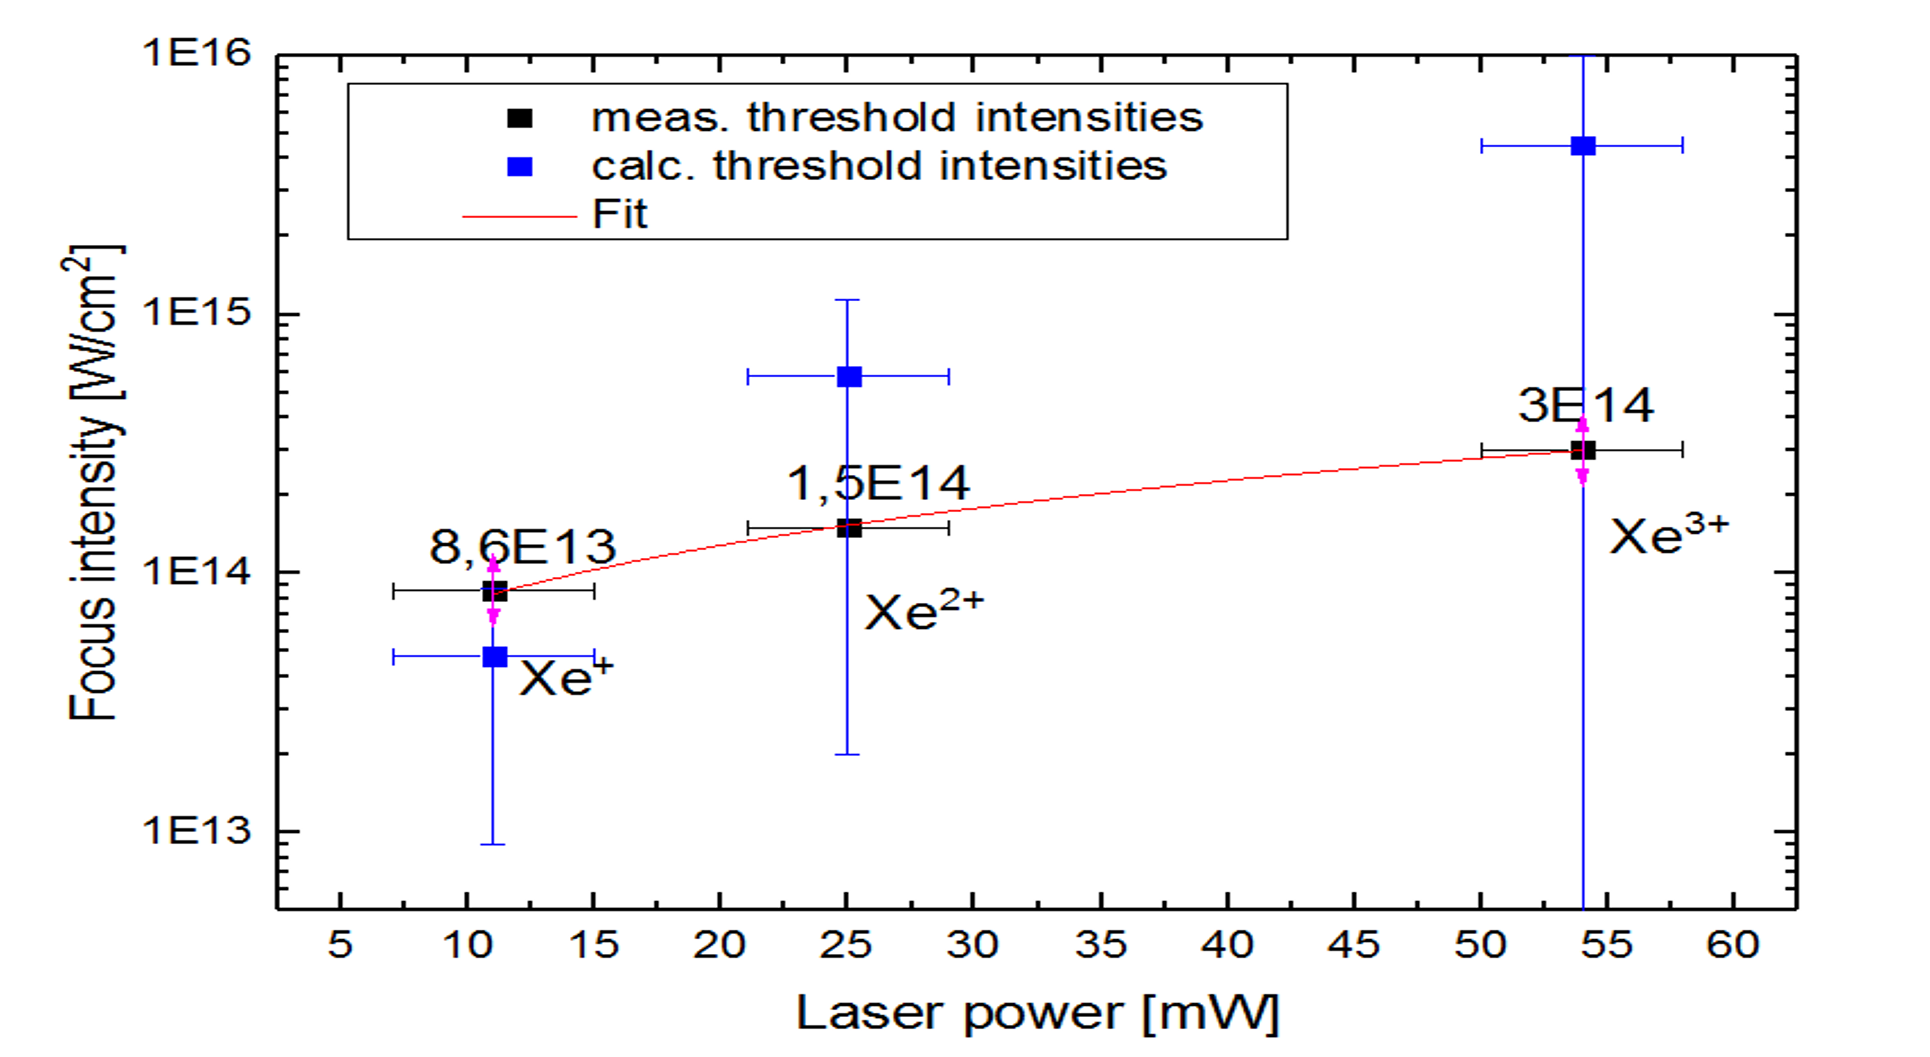
\includegraphics[width=10 cm]{../Images/Xeioncharges_intensitycalib.png} 
\caption[Xenon ion charge calibration for NIR] {Xenon ion charge calibration for NIR laser at three different power. On Blues the calculated threshold intensities and on black the experimental results for the power measured before the laser beam enter to the detection chamber.}
\label{fig:xeionchargecalib}
\end{figure}


\subsection{NIR. He Droplet Intensity scan.}

The laser system used at the Max plank instituted is a NIR laser at $800nm$ wavelength and a rate of $10Hrz$ and a $d_{pulse}=23$ fs pulse duration. Helium clusters at the same nozzle temperature $T_{nozzle}=12.2$ K and  backing pressure of $P_{0}=45$ mbar, were doped with Xenon at a fix doping level, with the a constant pressure measured in the oven chamber of $P_{oven}=2E-6$ mbar. This measurement where taken with a slightly smaller MCP-PHS arrangement of $d=42.2mm$ diameter of active area. At this nozzle temperature the Helium droplet have proximate $N=397390$ atoms before going through the oven chamber and its doped with $Xe_{dop}=134$ atoms, given a final number of He number of $N=386596$ atoms. The VMI voltages where set to VMIx2 and the MCP and PHS to $1250$ V and $4000$ V respectively. The camera was stablish to exposure time of $t_{exp}=1$ ms. 50000 pictures were taken for 7 different laser power, at $55,80,115,140,185,210$ and $240$ mW. 

\begin{figure}[h!]
\centering
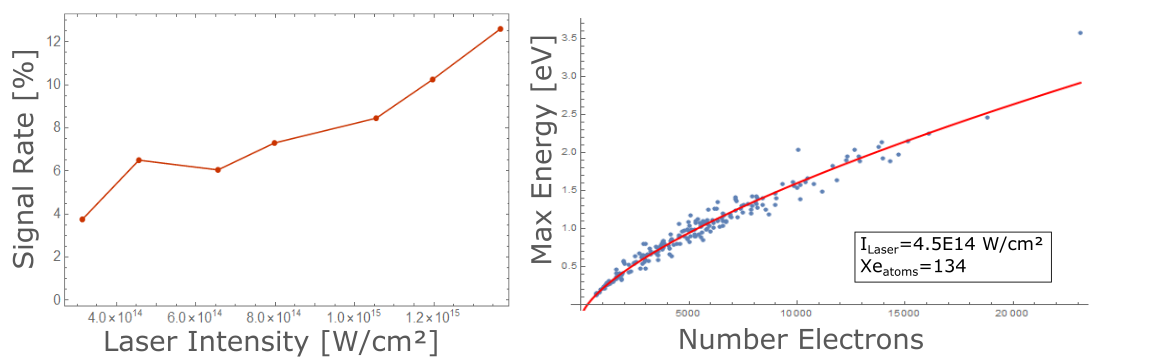
\includegraphics[width=16 cm]{../Images/results/NIR_He_intensityscan/signalrate_EnerDisttri.png}
\caption[NIR Helium, signal rate and energy distribution]{On left, signal rate for Helium droplets at different focus laser intensities. On the right the energy distribution of the droplet at 80 mW Laser power.}
\label{fig:NIRHEdistribution}
\end{figure}


As show on Fig. \ref{fig:NIRHEdistribution}, the signal rate depends strongly on the laser intensity, but even at lower intensities some coulomb explosion can be found. Although the percentage of pictures with signal decrease remarkably, we never find zero signal, it means that we have enough initial ionization to start the coulomb explosion. Despite the changing signal rate, we compare the Energy distribution depending on the number of electrons, a clear distribution on all signals is shown. In fig \ref{fig:NIRHEdistribution}, each blue point represents a individual picture, where the radius and brightness of each signal bloop is identified. Once all signal are analyzed, the distribution is plotted and fitted. The red line, is a fit based on $E_{max}= B \cdot n^{2/3}$, Eq. 3.12 where B is the B-Factor named on Eq. 3.13 and $n$ is the number of electrons, the $2/3$ factor is fix. The same process is done for each of the data sets at different laser intensities. All fits have the same tendency regardless the laser intensities, changing slightly on the B-factor. This in an important outcome meaning that the data fits quite well to our simple spherical electronic cloud model. As the B-factor is directly related to the density of the electronic cloud using Eq. 3.11 is possible to delimit the radii of the electronic sphere. In other words, according to this model, if we know the total number of electrons it’s possible to calculate the maximal energy that we can detect. 

\begin{figure}[h!]
\centering
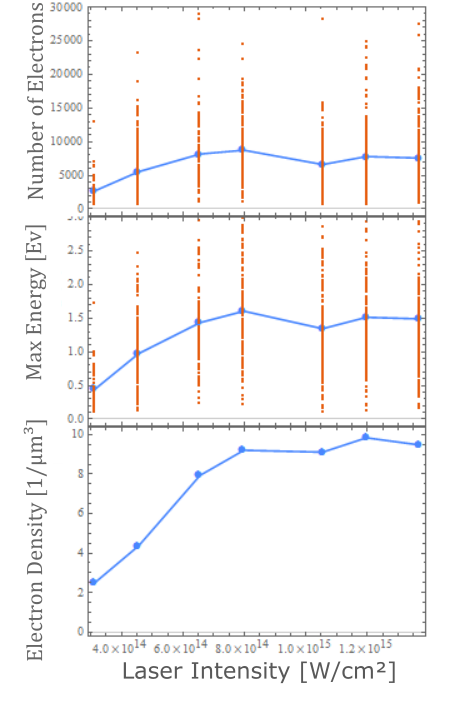
\includegraphics[width=7 cm]{../Images/results/NIR_He_intensityscan/histograms mean.png} 
\caption[NIR Helium. Histograms for Energy and electrons)]{On top, Mean number of electron for each of the data set at different laser intensities, on blue the mean values and in orange the individual results. On the center, mean value of the Max energy for different laser intensities. At bottom, the density (calculated from the B-coefficient) for the fit done in each of the data set.}
\label{fig:NIRHEhistograms}
\end{figure}

According to fig \ref{fig:NIRHEhistograms}, the mean number of electrons and the mean E$_{max}$, reach a maximum after $I=8.5E14$ W/cm$^{2}$ and keeps comparably constant for the following intensities. This result is not surprising because we don't expect large differences on the energies reached after the system is fully ignited, suggesting that after the beginning of the process, the coulomb explosion keeps a constant behavior. Fig \ref{fig:NIRHEhistograms}, bottom plot, shows the density of the electronic cloud, it is calculated from the B-factor of each fit function. It concur with our previous  assumption, it exhibit that there is a limit density that is not affected after certain intensity. Two assumptions can be done. First, the laser intensity play a fundamental role in given the starting condition to the nanoplasma formation but after a threshold, the laser does not influence in the final coulomb explosion any more. Second, a clear density limit is shown, it is possible that it is influence by this limitation of the laser on the process, but mostly it can be limited by the droplet size that was used in the experiment, as consequence, the biggest droplets are all expanding so in order to find bigger energy and densities we should use lower nozzle temperatures.  

 



\subsection{NIR. He Droplet size dependant.}

 For this data set, helium clusters at different nozzle temperatures, were doped with Xenon, with a doping pressure 2$E$-6 mbar measured in the doping chamber. The VMI were set to VMIx1 voltages and the MCP and PHS to 1250 V and 3400 V respectively. The camera was set to $\tau_{exp}=1$ ms exposure time. 50000 pictures were taken for 5 different temperatures, at 12.5 K, 13 K, 14 K, 16 K and 20 K. The data were analyzed using the data processing mentioned in chapter 3 to convert the bloop radius and its inner brightness to Maximal energy $E_{max}$ and Number of electrons $\#e-$.  Using the Hagena scale \cite{hagena_cluster_1972}, we can calculate a prediction of the total number of atoms before and after the doping. Table \ref{tab:NIRclustersize} shows the  mean number of atom per cluster to at the different nozzle temperatures and also its corresponding number of dopant. 

\begin{table}
\centering
\begin{tabular}{|l|l|l|l|}
\hline
\multicolumn{4}{|c|}{NIR  Helium Cluster Size (Ref)}                            \\ \hline
$T_{Nozzle} {[}K{]}$ &$ N_{He no dop}$ & $ N_{Xe atoms}$ & $N_{He}{[}atoms{]}$ \\ \hline
20                    & 32671          & 66        & 27362                      \\ \hline
16                    & 108424         & 199       & 92432                      \\ \hline
14                    & 222264         & 189       & 207173                     \\ \hline
13                    & 331040         & 149       & 319084                     \\ \hline
12                    & 509035         & 160       & 495949                     \\ \hline
\end{tabular}
\caption[NIR  Helium Cluster Size]{NIR  Helium Cluster Size}
\label{tab:NIRclustersize}
\end{table}


Fig. \ref{fig:NIRsrEnergy} shows the corresponding signal rate depending on the nozzle temperature. As shown, the biggest droplets contain the highest percent of signal compared to the small droplets. We need to take into account that the difference in size helps to the ignition of the process due the cross section for the interaction with the laser field also increase, so the ionization is easy. Furthermore, the larger the number of atom in the cluster the most electrons available to be detected. Once identified the radius and brightness of all the pictures, a Energy distribution is plotted. Fig \ref{fig:NIRsrEnergy} right, shows the energy distribution for the droplets sizes at 12.2 K. Each blue point represented a single picture, with the bloop radius and brightness transformed to energy and electrons. The red line, is a fit based on Eq. 3.12 where B is the B-Factor named Eq. 3.13 and $n$ is the number of electrons, the $2/3$ factor is fix to the fitting. The same process is done for the other nozzle temperatures, the fits have the same tendency for different droplet sizes and don't deferrer much between each other. For the B-factor at 12.5 K the corresponding electronic cloud density is around $\rho =2.2 [1/\mu m^{3}]$, what leads to a electronic cloud radius of  4.3 $\mu$m. 


 

\begin{figure}[h!]
\centering
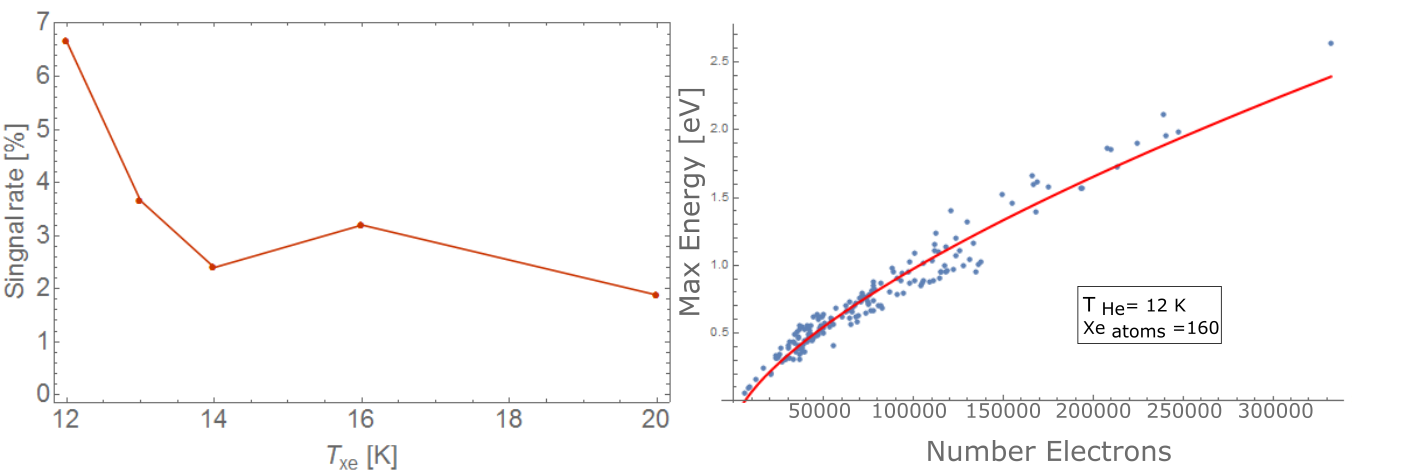
\includegraphics[width=14 cm]{../Images/results/NI_He_Dropletsize/signalrateee.png}
\caption[NIR He, Signal rate and Energy Distribution]{Signal rate and Energy Distribution for Helium droplet size scan. On the left, the signal rate for the different nozzle temperatures and on the right, an example of the energy distribution of the data set and it corresponding fit line. }
\label{fig:NIRsrEnergy}
\end{figure}


Figures \ref{fig:NIR2}. Shows the Mean $\#$e- and E$_{max}$ values for each size with their corresponding histograms. Hence, for example at 12 K, the energy histogram shows that exist counts for high energetic explosion, up to 4 eV, but the mean value of all the data is not higher than 2 eV. This behavior is also present for the other nozzle temperatures, where there exist a broad distribution for 13, 14 and 12 K, and presents a clear peak in the beginning of the plot for the higher energies.
Moreover, the number of electron in the system also rise with the size, for $T=$12.2 K the mean number is close to 160000 electrons, almost 10 time bigger than the smallest droplets. Similar as above, the 3 lower temperatures have a broad distribution than the smallest droplet, who show a peak at 10000 and 30000 electrons respectively. These results not just show that effectively, we are reaching different droplet sizes, but also that at these laser intensity the coulomb explosion is possible regardless the droplet size. At the same time, Showed that there are different droplet sizes and they form nanoplasma, so there in no doubt that their densities does depends on the coulomb explosion and the B-factor keep relatively constant, so the Energy for this NIR laser can be described by the density on it.



\begin{figure}[htb]

\captionsetup[subfloat]{farskip=2pt,captionskip=1pt}
\centering
\hspace*{\fill}%
\subfloat{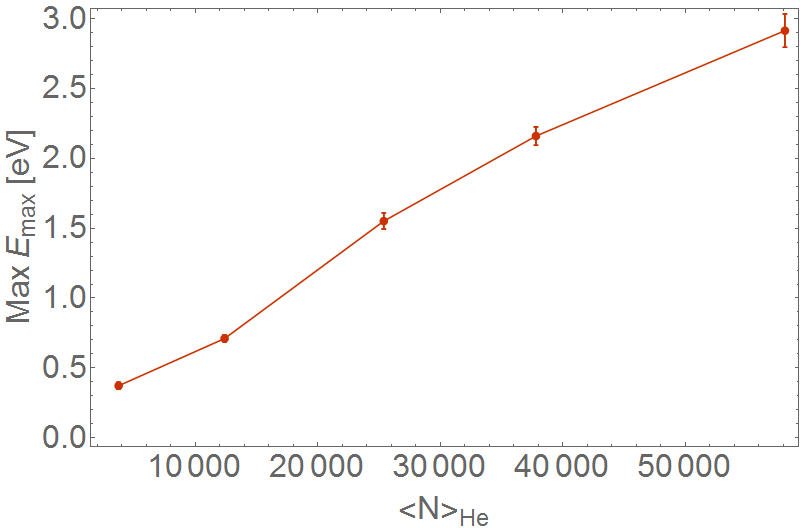
\includegraphics[width=0.35\textwidth]{../Images/results/NI_He_Dropletsize/MeanEnerg.png}
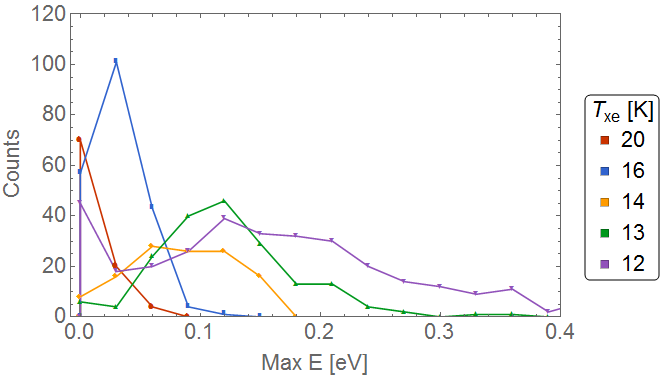
\includegraphics[width=0.4\textwidth]{../Images/results/NI_He_Dropletsize/Henerg.png}}
\hspace*{\fill}%

\hspace*{\fill}%
\subfloat{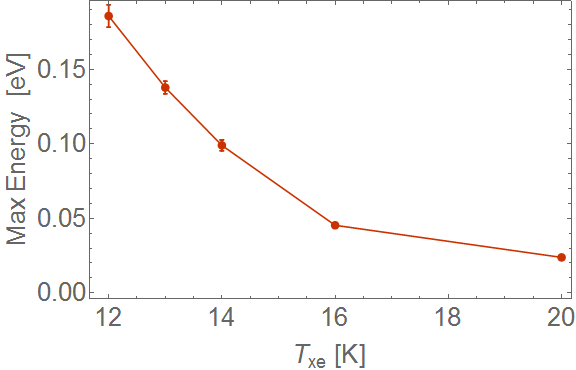
\includegraphics[width=0.35\textwidth]{../Images/results/NI_He_Dropletsize/MeanElec.png}
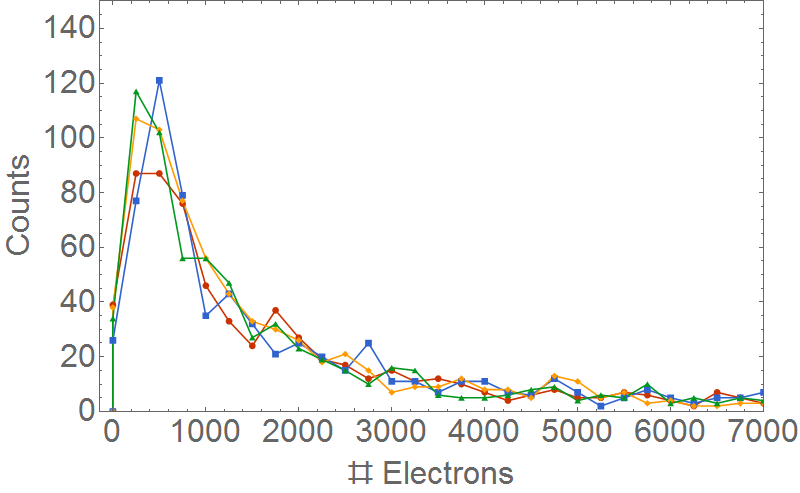
\includegraphics[width=0.4\textwidth]{../Images/results/NI_He_Dropletsize/Helec.png}}
\hspace*{\fill}%
\caption[NIR droplet size scan]{Mean Values and histogram for the droplet Size scan, on left the mean values for the different nozzle temperatures and on right, the respective Histograms counts for the binned data.}
\label{fig:NIR2}
\end{figure}



\section{Helium nanoplasma under MIR Fields }
 


Similar as the section before, Helium nano droplets doped with different alkaloids are described. Helium was expanded from a nozzle of $5 \mu m$ opening at a backing pressure of $P_{0}=30 bar$, using different nozzle temperatures to produce a jet of helium nano droplets. This beam is doped by a Xenon gas, when passing through a gas doping cell in the doping chamber or Calcium atom when it pass through the oven. Therefore, the mean dopant cluster size is determined by the xenon pressure in of the gas doping cell, which is controlled by a high-precision needle valve and the oven temperature. The flight distance through the gas doping cell is $30mm$. The MIR laser pulses are orthogonal to the cluster beam through a vacuum window into the chamber and focused into the cluster beam by a focusing mirror.
The laser intensity in the focus during the measurements was in average $2.5E14$ W/cm$^{2}$ at a maximum power of $P\sim 9$ W , it had a minimum pulse duration of $t_{pulse}=45$ fs and a rate of 10 KHz. The laser power depends on the pulse duration because the total pulse energy needs to be distributed on time, in each specific case we will denote the power when it changes. The polarization of the laser field was orthogonal to the spectrometer axis. The electronic signals were recorded with the Basler CCD camera at a minimal exposure time $t_{Exp time}=45 \mu$s triggered with the TOF as explained in chapter 3, this process grants the single shot signal. The camera is focused on the MCP-PHS arrange that makes the electron signal visible. 


Because, in general, not all laser shot hits a cluster or generates a plasma explosion,  most of the data sets presented next have a low signal rate, in order to have representative statistics, in each experiment were taken 10000 pictures, from those, about less than $10\%$ had signal. Most of the VMI signal had the expected circular aspect except for the larger size droplets, with the donut shape.

The data identification and process follows chapter 3, and in case of the donut shape pictures, this data were analyzed independently. In each signal picture the maximum blob radius and its respective inner brightness are identified and transformed into number of electrons and max energy. Each set of data is different, so once we analyses all the pictures a distribution function can be plotted.

\subsection{MIR. Helium Droplet size dependence.}

For this data set, He clusters at different nozzle temperatures, were doped with Xenon at a pressure of $0.0060$ mbar measured in the gas doping cell. The voltages were set to VMIx1  and the MCP and PHS to $1600$ V and $4000$ V respectively. The camera was set to minimum exposure time and the trigger system was used. 100000 pictures were taken for 4 different temperatures, at 10.6 K, 11 K, 12 K and 12.5 K. The data where evaluated once more as last section, demonstrating that the Trigger system worked efficiently. As result, it was shown that even for this high repetition laser rate, single shot signals can be achieved. The TOF signal work as a reference to identify the single explosion, and then each individual VMI picture is treated as follows. Fig \ref{fig:tofhe} shows a mean TOF for the measurement at 10.6 K. As we can see, there is a large amount of water and a small peak for hydrogen still in the vacuum chamber, this remain gases affect especially for the background. It is shown that Helium is effectively ionized due the peak at He$^{+}$ but on contrast no He$^{2+}$ signal was identify.

\begin{figure}[hbtp]
\centering
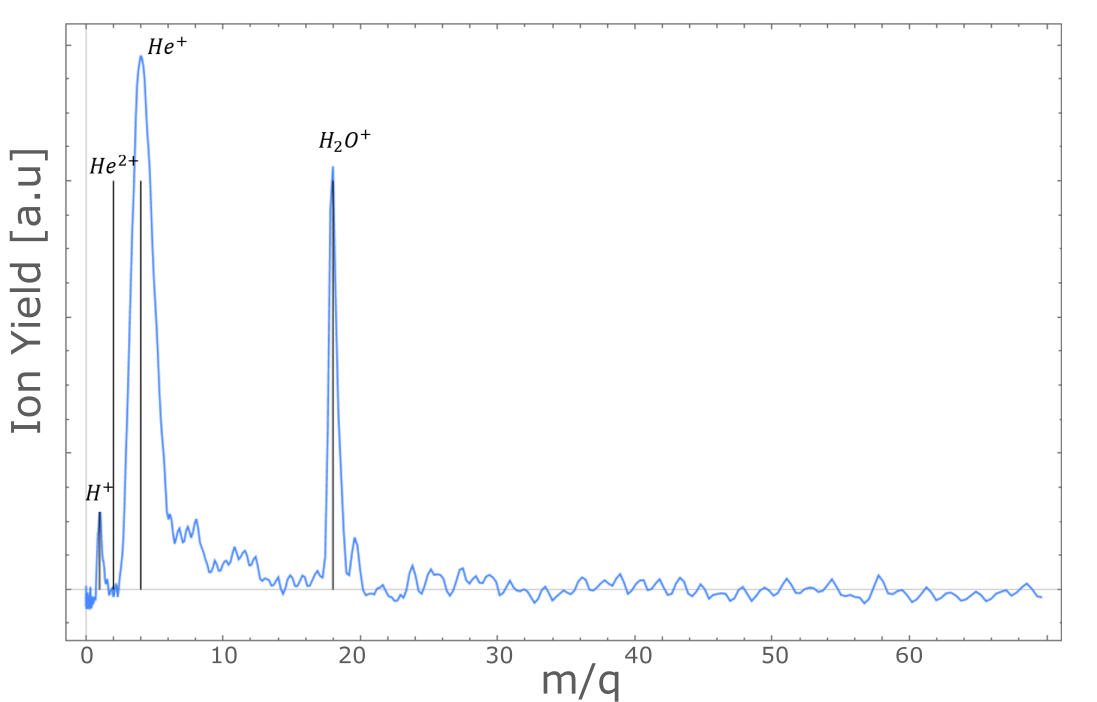
\includegraphics[width=0.7\textwidth]{../Images/TOF-10k6.png}
\caption[MIR TOF spectra He ]{Mean TOF spectra for He at 10.6 K}
\label{fig:tofhe}
\end{figure}

Using the Hagena scale \cite{hagena_cluster_1972}, we can calculate a prediction of the total number of atoms before and after the doping. Table \ref{tab:clustersize} shows the mean number of atom per cluster to at different nozzle temperatures and also its corresponding number of dopants. As reference for the cluster size scaling law, we used data at $P_{0}=50$ bar and temperatures similar to the experiment. 

\begin{table}[t]
\centering
\begin{tabular}{|l|l|l|}\hline
\multicolumn{3}{|c|}{Cluster Size reference}                                                             \\\hline
T$_{Nozzle}$ {[}K{]}  & N$_{Xe atoms}$ & $\langle$N$\rangle$ $_{He atoms}$ \\ \hline
10.6                  & 220     & 2.80E5                      \\ \hline
11                    & 192     & 2.29E5                      \\ \hline
12                    & 138     & 1.42E5                      \\ \hline
12.5                  & 119     & 1.13E5                     \\ \hline
\end{tabular}
\caption{cluster size reference}
\label{tab:clustersize}
\end{table}


\begin{figure}[h!]
\centering
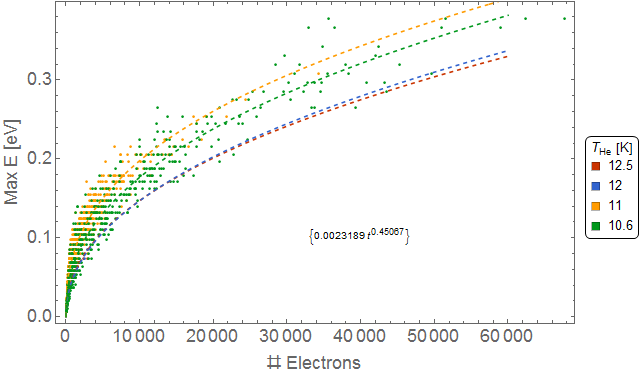
\includegraphics[width=0.7\textwidth]{../Images/results/Mir_He_Dropletsize/fits.png} 
\caption[He-Xe droplet size distribution]{Maximal Energy distribution on the number of electrons. On colors the different nozzle temperatures, the smallest droplets (12 K,12.5K) presents few signal images and can be seen behind the yellow and green  points in the left-bottom of the graphic.  The dash line are the fit curves.}
\label{fig:energdistributionHeXeSize}
\end{figure}

Fig \ref{fig:energdistributionHeXeSize} shows the energy distribution versus the number of electrons. As we can see, most of the data point lay on the bottom-left of the graph at lower energies, but the distribution also show signals with energies up to 0.4 eV and 50000 electrons collected, this signals comes from the most energetic coulomb explosions, and we can clearly see that the bigger the droplet the  brightness we can get. Due the few signal for the 2 higher temperature we discard the 2 fit lines, moreover, for the others, its fit lines are in a relatively good concordance to the data using Eq. 3,13 as a guide, we find a B-factor $B=0.00305103$ and a factor $k=2/5$. 

On one hand, the first big different with the experiments with the NIR laser, is this non correlation to the uniformly charged Cloud model, especially in the exponent $k$, that changes from 1/3 to 2/5. There is no theoretical background that can predict this behaviour but as the exponent is closely linked to the geometry of the cloud, we can assume the fits does not agree because the  big droplets are not perfectly spherical, so for example, as they are liquid, the droplets could turn in an ellipsoidal. This new exponent is persistent in all the fit for the MIR experiments in helium. On the other hand, as explained, the B-factor is directly related to the density and in consequence to the radius of the electronic cloud. Given B, we obtain approximately $R_{cloud}=85$  $\mu$m, a radius three order of magnitude bigger that the initial cluster, that for example at 11 K have $R_{cluster}=13$ nm.

\begin{figure}[h!]
\centering
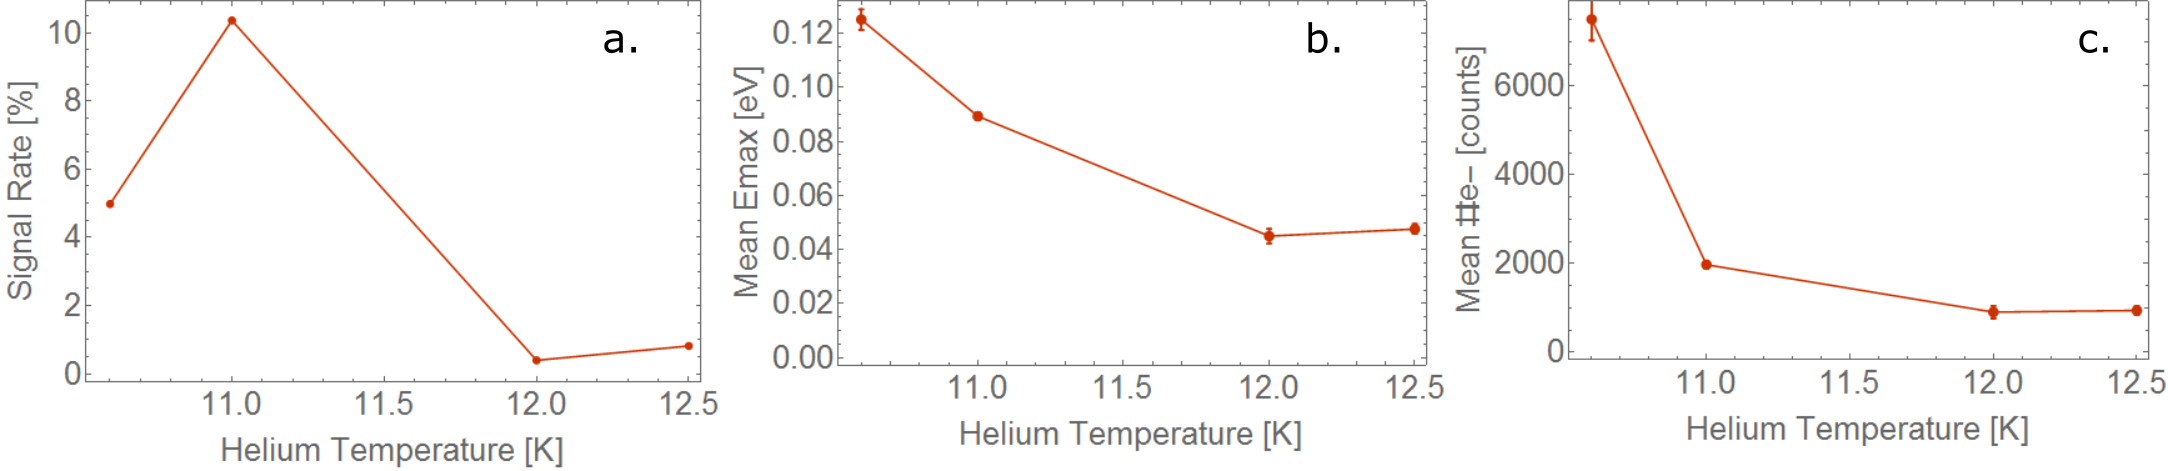
\includegraphics[width=16 cm]{../Images/results/Mir_He_Dropletsize/signalrates.png} 
\caption[He-Xe, signal rate droplet size]{Figures a, shows the signal rate in percentage of the pictures with signal depending on the nozzle temperature, B and c. show the mean of the number of electrons and the Max energy for each point respectively.}
\label{fig:sigratedropletsize}
\end{figure}

Fig \ref{fig:sigratedropletsize} presents the Signal rate and the Mean values for the number of electrons and max energy depending on the temperature of the nozzle. As shown the figure, for the biggest droplet (points to the left) we got the largest signal rate at 10.6 K and 11 K and immediately for the smaller droplet the rate decrease drastically, same tendency is show b and c making clear that plasma is easier to ignite at lower temperatures. Therefore, as more electrons and energy are detected while the signal rate increase, we assume that the nanoplasma formation is more efficient for larger droplets. The drop on the signal rate at 10.6 K compared to the 11 K can evidence a loss of efficiency for the laser to ionized even bigger droplets. In other words, After certain droplet size, is more difficult to ignite the plasma.  Unfortunately, no other measurement where taken at lower temperature to confirm if this is a statistical event or a real tendency.


\begin{figure}[h!]
\centering
\begin{subfigure}[l]{0.49\textwidth}
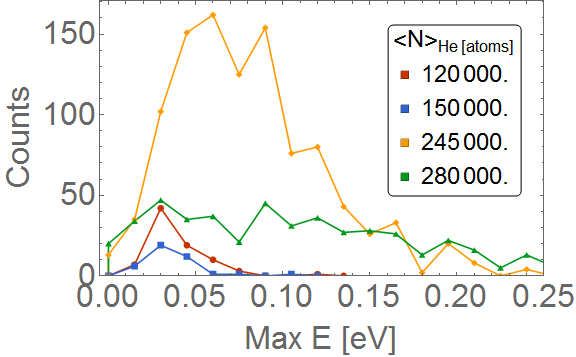
\includegraphics[width=1\textwidth]{../Images/results/Mir_He_Dropletsize/Henerg.png}   				\end{subfigure}
\begin{subfigure}[l]{0.49\textwidth}
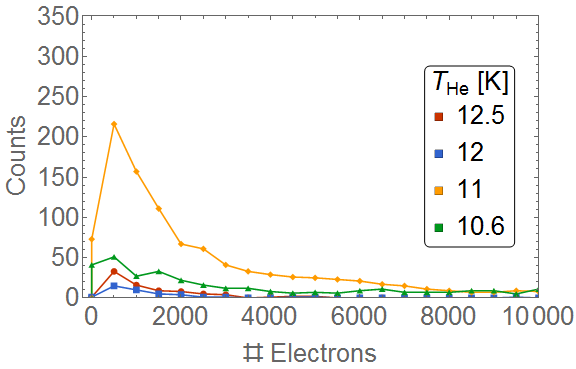
\includegraphics[width=1\textwidth]{../Images/results/Mir_He_Dropletsize/Helec.png} 
\end{subfigure}
\caption[MIR He droplet scan histograms]{On the left, The hitogram for max energy and on rigth, the histogram for number of electrons.}
\label{fig:histodropletsize}
\end{figure}

Fig \ref{fig:histodropletsize} shows the histogram of the $E_{max}$ and  $\#$e- for the different temperature. On one hand, in the $E_{max}$, the first peaks describe that most of the droplets achieve energies between $0.05$ and $0.1$ eV, decreasing rapidly after that. On contrary, the biggest droplets have a more broaden distribution that the higher temperatures. One interesting feature is that there exist an offset from zero energy for all temperatures which can be related to a minimal energy needed to ignite of the plasma autonomous of the cluster size.  Furthermore in the $\#e-$, a broader distribution is show, a huge density is found for droplets with less than 2000 electrons, having a drastic decrease. It show a clearly distribution where the main average size of the droplet is small,  but without discarding that some individual points at a huge number up to 80000$e-$, this shows that at bigger droplet also the high the chance to have more populated electronic clouds.



\subsection{MIR. Helium-Argon doped.}

In this data set, He clusters were doped with Argon at different gas doping pressures. Helium was produced at a nozzle temperature $T_{nozzle}= 11$ K and ignited by the MIR laser pulse, the VMI were set to VMIx1 voltages and the MCP and PHS to 1700 V and 4000 V respectively. The camera was set to $t_{exp}$=50 $\mu$s exposure time what means the data was not correlated with the same trigger. The exposure time was modified due the low signal rate, nevertheless the information will be still evaluate in the same way  as before, taking into account that signal rate was so low that is possible to have single shot.  100000 pictures were taken for 3 different doping pressures, at $2E-4, 6E-4$ and $12E-4$ mbar measured in the gas doping cell. 

\begin{figure}[h!]
\label{fig:HeArEnergydistr}
\centering
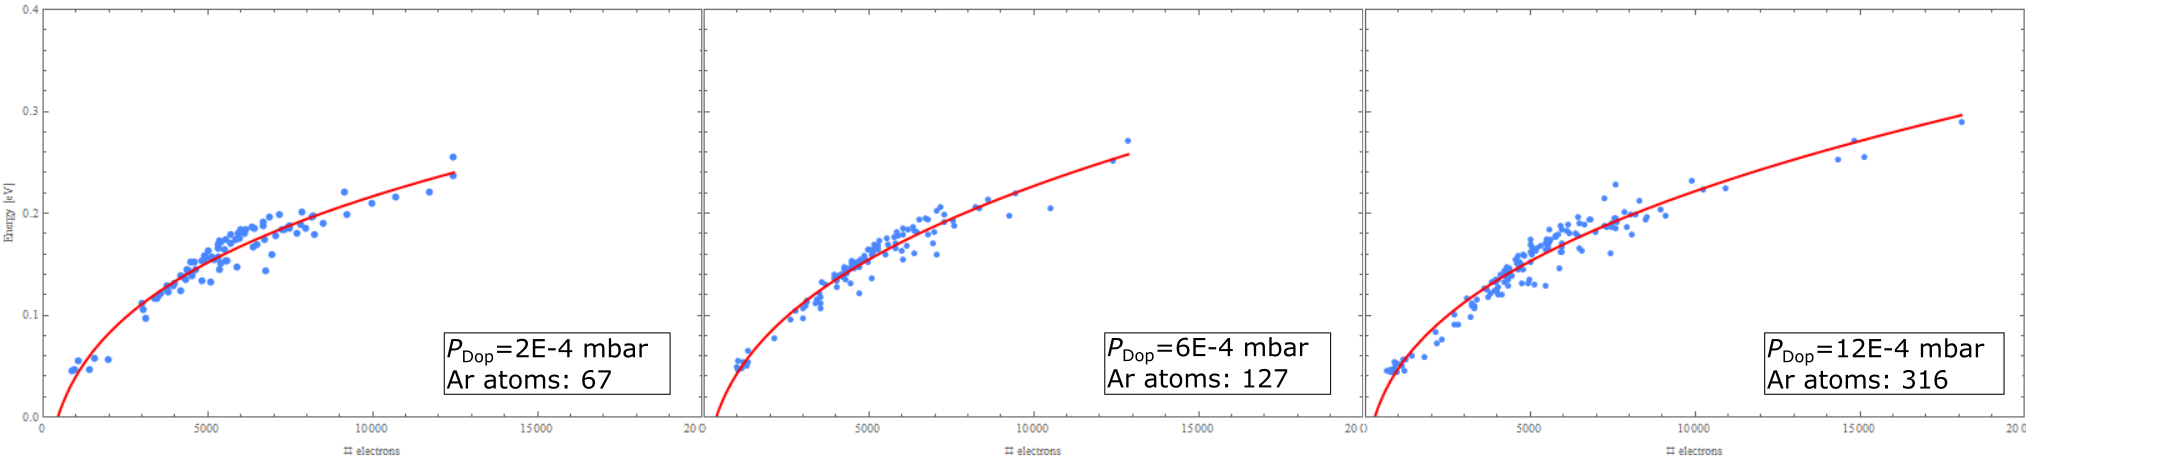
\includegraphics[width=17cm]{../Images/results/MIR_He_ArDop/pointfits.png}
\caption[He-Ar Dop distribution]{Energy distribution for He  cluster at different Argon doping levels}
\label{fig:HeArEnergydistr}
\end{figure}

Fig \ref{fig:HeArEnergydistr} shows the maximal energy distribution for three different pressures and it corresponding number of dopant. As mentioned, the signal rate for this data set was quite low showing that the efficiency for this doping is lower than for Xe. In red the fit done with the same fitting parameters than above with a B factor $B=0.09714$ what gives us a mean radius for the electronic cloud of  $R_{cloud}=$92.4 $\mu$m, quite proximately in the same order of magnitude to the data set above. For the Exponent, it was set as a free parameter given in general $k=2/5$ as well. 

\begin{figure}[h!]%\centering
    \begin{subfigure}{0.3\textwidth}
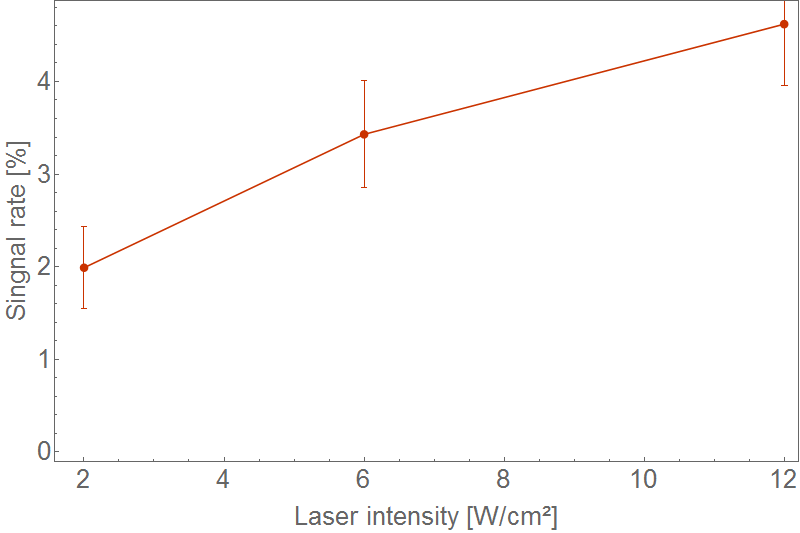
\includegraphics[width=1\textwidth]{../Images/results/MIR_He_ArDop/signalrate.png}     
    \end{subfigure}

   \begin{subfigure}{0.34\textwidth}
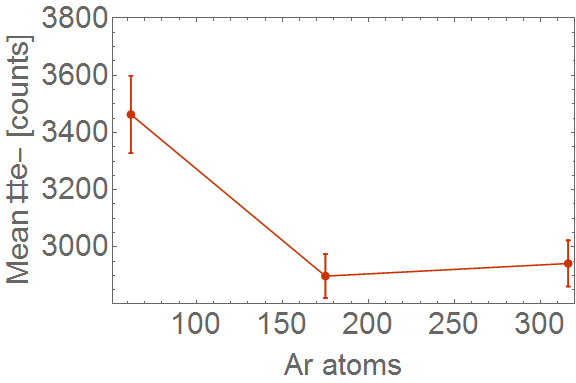
\includegraphics[width=1\textwidth]{../Images/results/MIR_He_ArDop/Meanelect.png}     
    \end{subfigure}
 
    \begin{subfigure}{0.34\textwidth}
    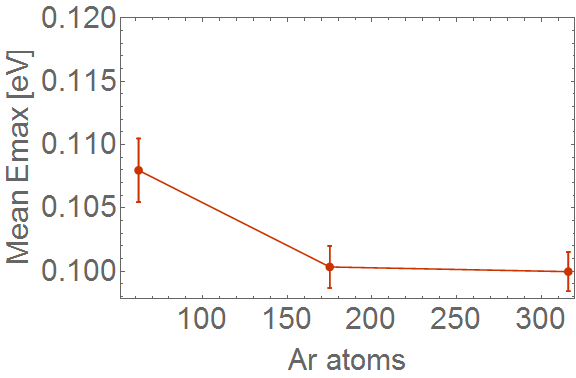
\includegraphics[width=1\textwidth]{../Images/results/MIR_He_ArDop/Meaneneg.png} 
\end{subfigure}


\caption[MIR He-Ar doping, signal rate and histograms]{On the left, the signal rate for the He-Ar doping. Center and right, are the mean values for the number of electrons and max energy respectively}
\label{fig:He-Armean}
\end{figure}

Fig \ref{fig:fig:He-Armean} shows the signal rate and Mean values for the data. On the signal rate is clear that the amount of dopant increase the efficiency of the plasma, going from a low rate up to 5$\%$. Combined to the Mean values results, we can deduce that the efficiency for small droplets ignition also improve at higher doping. As seen before, the mean values for number of electrons and energy decrease while the signal rate increase. evidencing that there are more small droplets explosion detected.
  

\subsection{MIR. Helium-Water scan.}

The Nanoplasma explosion process starts when the dopant gives electrons to the cluster in order to ignite the plasma. One of the most commune and available dopant is water, not just because it’s easy to get in the lab but also because it’s also difficult to remove from the vacuum chamber. Even in our best vacuum, experiments usually contained few traces of water. In addition, at Mid-Infrared, water have a special resonance that could be advantageous because it will withstand a faster ionization and in consequence, a better creation of the plasma. This data set was taken with He droplets at $T_{nozzel}=11$ K doped with water. A small drop of water were located into the entrance of the needle valve, to achieve a controlled doping. The pressure at the gas doping cell was varied in order to perform several doping levels. The camera was set to $t_{exp}=120$ ms so single shot was not enable. The voltages were set to VMIx1 and the MCP and PHS to $1750$ V and $4000$ V respectively. 100000 pictures were taken for 5 different doping pressures, at 1$E-$4, 2$E-$4, 3$E-$4, 6$E-$4 and 12.5$E-$4 mbar. 

\begin{figure}[h!]

\centering
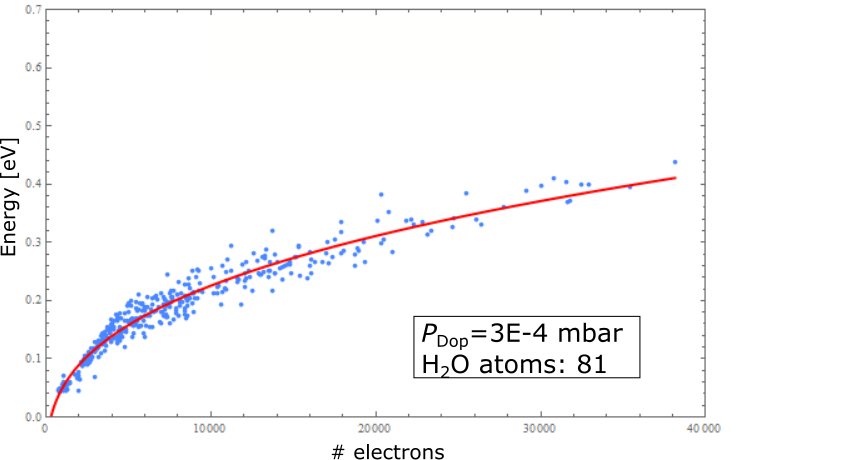
\includegraphics[width=0.7\textwidth]{../Images/results/MIR_He_waterDop/Energyfit.png}
\caption[He_h2O energy distribution]{Plot of the $E_{max}$ and $\#e-$ distribution for He doped with water at 0.00120 mbar, on red the fit for the point.}
\label{fig:He-waterEnergydistrib}
\end{figure}

Fig. \ref{fig:He-waterEnergydistrib} shows the energy distribution for just one of water pressures. On blue are the points that represent the E$_{max}$ and $\#e-$ for an single signal picture and on red the fit based on the Eq. 3.12. For the water doping pressures the distribution looks almost the same, just changing in general the signal rate as shown in Fig. \ref{fig:Hewaterhistograms}. The fit function is used to find the B factor, obtaining for this example $B=0.01509$, that gives a radii for the electron cloud of $R_{cloud}=92.4 \mu$m, with an exponent factor $k=2/5$. 

Fig \ref{img:sigratedropletsize} presents the rates for signal as the Mean number of electrons and max energy depending on the temperature of the nozzle. As shown, for the biggest droplet (points to the left) we got the largest signal rate at $10.6$ K and $11$ K and immediately for the smaller droplet the rate decrease drastically, same happens in the mean signals where the biggest droplets are the once that reach the higher counts. The measurements show that with decreasing nozzle temperature, therefore increasing droplet size, the frequency of single-shot signals increases, and higher kinetic energies can be detected.

\begin{figure}[ht]%\centering
    \begin{subfigure}{0.3\textwidth}
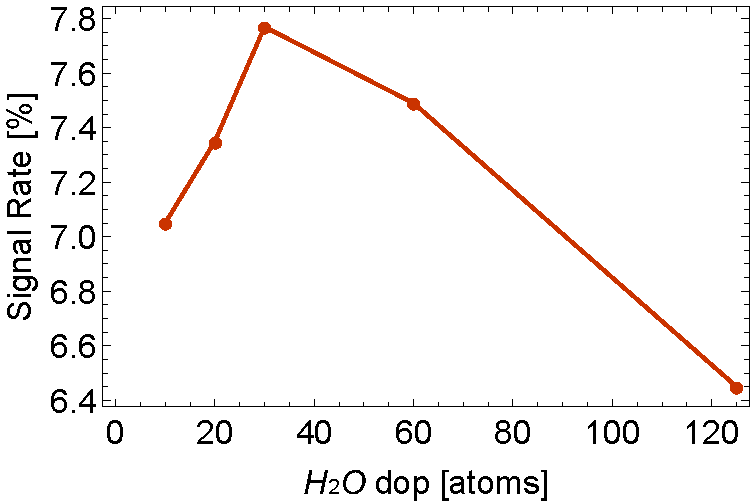
\includegraphics[width=5cm]{../Images/results/MIR_He_waterDop/results/MIR_HE_water_Signalrate.pdf}     \caption{Signal rate}
        \label{fig:HeArhistograms-electr}
    \end{subfigure}
\hfill%\hfill
   \begin{subfigure}{0.3\textwidth}
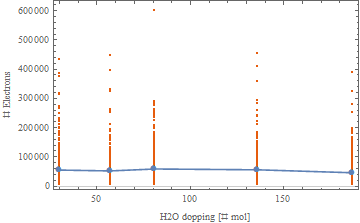
\includegraphics[width=5cm]{../Images/results/MIR_He_waterDop/results/Nelc_dopp.png}    
    \caption{$\#$Ne- histogram}
        \label{fig:HeArhistograms-electr}
    \end{subfigure}
\hfill%\hfil
    \begin{subfigure}{0.3\textwidth}
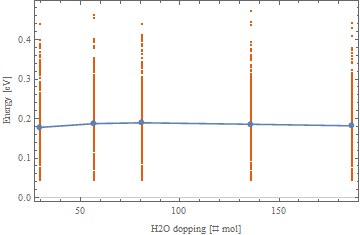
\includegraphics[width=5cm]{../Images/results/MIR_He_waterDop/results/Kener_Dopp.png}     \caption{$E_{max}$ histogram}
    \label{fig:HeArhistograms-energ}
\end{subfigure}
\hfill%\hfil
     \caption[MIR He-water doping, signal rate and histograms]{On left, the signal rate for the He-water doping, B. and C. are the histogram of the point for the main  number of electrons and energies respectively}
    \label{fig:Hewaterhistograms}
\end{figure}

As we show, under the correct doping levels and He cluster sized, water molecules are a great dopant for Helium clusters under MIR laser pulses. The nanoplasma reach high energy states as well as a huge radius for the electronic cloud, reaching mean of electrons detected up to 70000. The mean values in the energy or electrons does not depend on the doping, as already described in the other experiments, once the ionization process ignites the plasma  the final result does not present variations.


\subsection{MIR. Helium-Water Intensity scan.}

Similar to the experiment done in Heidelberg with the NIR laser pulse. A intensity scan was performed in order to see the effects of the laser system on the coulomb explosion. The laser system used at ELI-Alps is at $3200$ nm wavelength and a rate of $100$ KHz and a $\tau_{pulse}=45$ ps pulse duration. Helium clusters at the same nozzle temperature $T_{nozzle}=11$ K and  backing pressure of $P_{0}=30$ mbar, were doped with Water at a fix doping level $P_{dop}=1E-4$mbar pressure measured in the gas doping cell. At this nozzle temperature the Helium droplet have proximate $N=244647$ atoms before going trough the oven chamber and its doped with H$_{2}$O$_{dop}$=56 atoms, given a final number of He number of $N=215972$ remaining atoms. The VMI voltages where set to VMIx1 and the MCP and PHS to $1750$V and $4000$V respectively. The camera was stablish to exposure time of $t_{exp}=34 \mu$s. 100000 pictures were taken for 6 different laser power, at $2, 4, 6, 7, 8$ and $9.5$ W, measured before the laser beam enters to the detection chamber and its back focus by the mirror. 

\begin{figure}[h!]
\centering

\hspace*{\fill}
{ 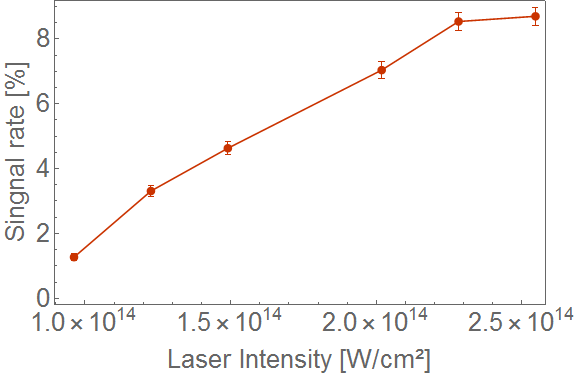
\includegraphics[width=6cm]{../Images/results/MIR_He_waterIntensityscan/sigRate.png}} \hfill {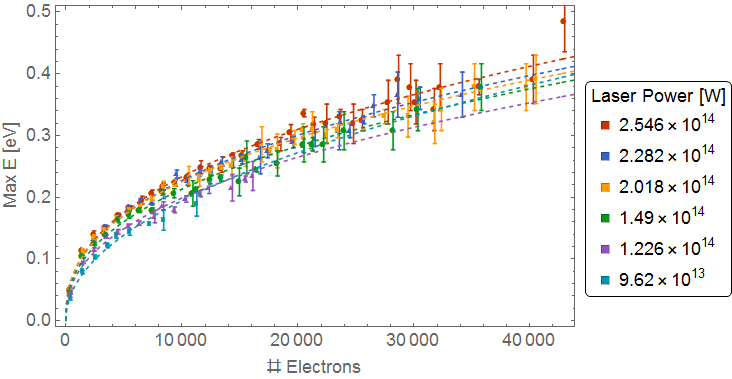
\includegraphics[width=7.5cm]{../Images/results/MIR_He_waterIntensityscan/binned.png}}
\hspace*{\fill}
\caption[MIR He intensity scan]{On the left, Signal rate for the He-Water laser intensity scan. On the right, the binned energy distribution for the maximum Energy respect to the number of electrons. In colors are the different laser power transformed to focused intensities. }
\label{fig:mult1}
\end{figure}

Having the laser power, the intensity can be calculated for each laser power using the Xe cut off calibration. The legends in Fig.\ref{fig:mult1} shows the different laser intensities calculated for each of the laser power used in the experiment. Fig \ref{fig:mult1} shows the signal rate and the energy distribution for the coulomb explosion, the signal rate is taken as the percentage of pictures with relevant signal in the data set, once the pictures are identified the radius and internal brightness is find, similar to the results above. Each of the color points in energy distribution plot are the binned data in number of electrons every 1000, the error bars correspond to the standard derivation in the distribution. The points with the lower power, have high error due the signal rate at this intensities is extremely low to have good statistics. The dashed lines are the corresponding fits to each of the intensities taken, the lines for the two lower intensities are not plotted due the low statistics on them. The fitted line was done according to Eq. 3.12 as usual, the fits actually preserve the same tendency where the $k$ factor was keep constant to $2/5$, and the B-coefficient was calculates in order to find the density of the electronic cloud. For example, at the highest power P=9.5 W, B=0.0101, giving an estimated for the density of $\rho= \mu m^{-3}$$ and a radius of R=8 $\mu$m.
The signal rate shows that the laser intensity plays a fundamental role in the ignition of the process, at lower intensity, less probable to find signal. But at the same time we can identify that after the intensity go up to $2E14$w/cm$^{2}$ the process starts to keep in a constant rate, that suggest there exist an intensity threshold to overcome so the plasma formation will not be affected by the extra intensity radiated. this could be attribute to the ionization process, As known certain energy need to be transfer to the dopant to ionized, but once the a intensity is reach all dopant will be completely ionized, so there is no need to use powerful beams. 


\begin{figure}[htb]
\captionsetup[subfloat]{farskip=2pt,captionskip=1pt}
\centering
\hspace*{\fill}%
\subfloat{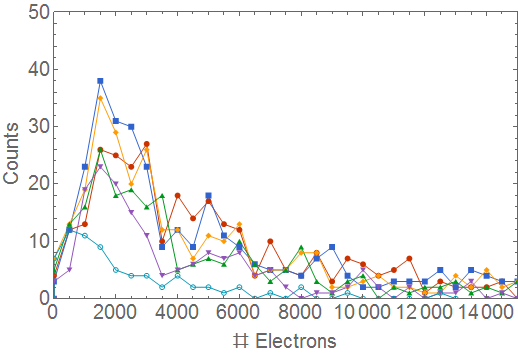
\includegraphics[width=0.4\textwidth]{../Images/results/MIR_He_waterIntensityscan/Helect.png}}
\subfloat{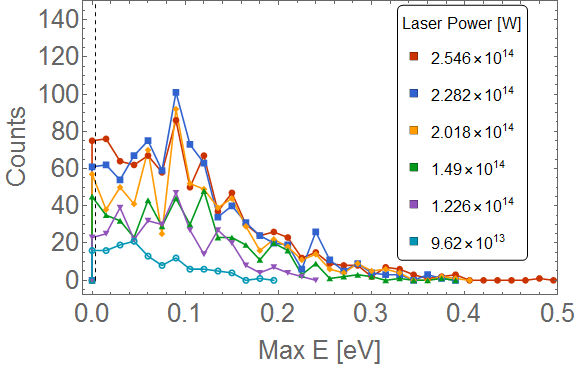
\includegraphics[width=8.0cm]{../Images/results/MIR_He_waterIntensityscan/HEnerg.png}}
\hspace*{\fill}%
\hspace*{\fill}%
\subfloat{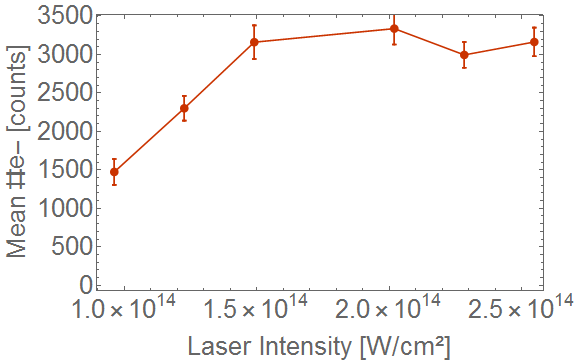
\includegraphics[width=0.4\textwidth]{../Images/results/MIR_He_waterIntensityscan/Meanelec.png}}
\subfloat{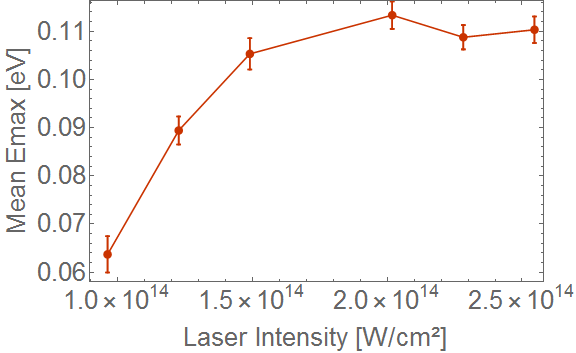
\includegraphics[width=0.4\textwidth]{../Images/results/MIR_He_waterIntensityscan/Meanenerg.png}}
\hspace*{\fill}%
\caption[MIR He pulse scan. Mean values and Histograms]{On the top, Histograms for number of electro (left) and maximal energy (rigth) for the diferent pulses. On bottom, The mean $\#$e- and energyy from the energy distribution for ecah pulses}
\label{fig:MIRwaterintenhisto}
\end{figure}


 Fig. \ref{fig:MIRwaterintenhisto} show two plot corresponding to the Mean of energy and number of electrons for each data set at it corresponding intensities and also the histograms with the respectively distributions. On Bottom, the mean values of $\#$e- and E$_{max}$, shows a disposal similar to the signal rate, the more intense the laser pulse the more energy and electrons can be found. The means values start to rise in a fast way on left but once it reach the 3 best intensities the divergence decrease and changes are less noticeable. On bottom, on the histogram a clear distribution is present. On the bottom left, we can deduce that exist a predominant range of energies, it is clearly mark that for all intensities most of the electrons reach a max energy between 0.1 $\rightarrow$ 0.2 eV, decreasing the counts drastic after 0.25 eV, it’s important to take into account that for the smallest bloops signals, the lower energetic points are not taking into account because the radius finder can`t spot signals with less than 6 pixels of radius. Furthermore, on the right histogram, most of the data is distributes in the peak near to 2000e-, having stiff rise from zero to 100 and a slower decrease after 4000e-, the counts for bigger electronic clouds  decrease drastic for bigger numbers. A second trend that can be sift is that the peak count decrease with intensities, as shown, although most of the peaks lay close to the same number, the counts, the dark blue line correspond to the higher intensity which have the higher counts, the higher the intensity the higher the counts, until reach the red line and light blue line. This counts depends directly from the signal rate , but in the Mean Values we can spot that the Energies and the number of electrons does shift their distribution to bigger values with the intensities, it means that this high power allowed to reach bigger nanoplasmas that will denote in high energy numbers too.
 
 
 
\subsection{MIR. Helium Pulse duration dependency}
 
 One of the advantage of the laser system in ELI-Alps, is the possibility to change the laser pulse duration. In this data set, we present the result for the energy distribution of helium cluster doped with Xenon under different pulse duration.  Helium clusters at the same nozzle temperature $T_{nozzle}=10.5$ K and  backing pressure of $P_{0}=30$ mbar, were doped with Xenon at a fix doping level $P_{dop}=2.4E-4$ mbar pressure measured in the gas doping cell. At this nozzle temperature the Helium forms big clusters, with approximated $N=3150000$ atoms before going through the oven chamber and its doped with Xe$_{dop}$=75 atoms. The VMI voltages where set to VMIx1 and the MCP and PHS to $1600$V and $4000$V respectively. The camera was stablish to a exposure time of $t_{exp}=34 \mu$s. A first averaged mode signal was taken as a guide to the eye and after 100000 pictures were taken at 4 different pulse duration, at $65, 120, 200$ and $250$  fs, measured by the ELI-laser personal supporting us in the experiment, using FROG technique.
In the beginning of the experiment, we notice that the laser pulse have a dependence with the laser power,   longer pulses results in a weaker power. Table \ref{tab:pulsepower} resume the laser power obtained for each of the pulse duration. Fortunately the intensities didn't defer much and the intensities obtained are farther that the threshold to start the coulomb explosion as seen in the intensity scan above.
  
   
\begin{table}[]
\centering
\label{tab:pulsepower}
\begin{tabular}{|l|l|c|}
\hline
Pulse duration {[}fs{]} & \multicolumn{1}{c|}{Power{[}mW{]}} & Laser intensity {[}W/Cm\textasciicircum{}\{2\}{]} \\ \hline
65 & 8.8 & 1.5E14 \\ \hline
120 & 9.7 & 8E13 \\ \hline
200 & 9.8 & 5E13 \\ \hline
250 & 9.2 & 3.9E13 \\ \hline
\end{tabular}
\end{table}


Fig. \ref{fig:sigenergdistpulse} shows the signal rate and the Binned energy distribution for all the different pulses. As shown, the signal rate have a mark dependence on the  pulse duration, showing on left a big signal rate of almost 20$\%$  and decreasing constantly until  the longer pulses decrease down to  10$\%$.  This behavior is suspected because, as already mentioned, even the output power of the laser tends to remain continuous and once we stretch the pulse, the energy gets redistributed, so the laser field interacting in the ionization process is weaker, hence, the coulomb explosion ignition probability decrease. At the same time, on the energy distribution plot an interesting results are exhibited.  As usual all point represent the $\#$e- and E$_{max}$ of a single picture and the dashed line is the corresponding fit for each laser pulse following Eq. 3.12, letting the exponent and B-factor variable. In general all  plasmas behave in similar way, the fit lines goes almost parallel to each other and display the same B-factor  of 0.000179 that leads to a Radius for the electronic cloud of almost 500 $\mu$m with a factor of $2/5$. This similarity in the B-factor could represent that the energy distribution actually doesn’t seen affected by the laser pulse duration.



\begin{figure}[h!]
\centering

\hspace*{\fill}
{ 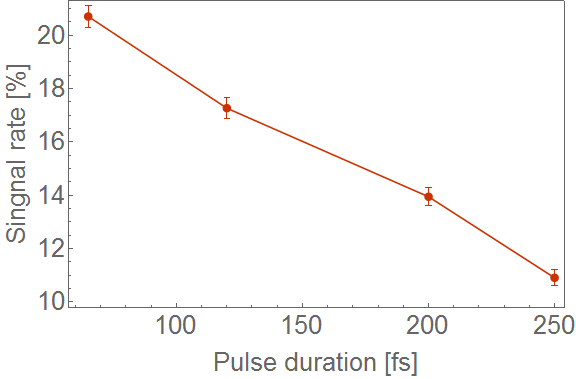
\includegraphics[width=6cm]{../Images/results/MIR_He_pulsescan/raw/signalrate.png}} \hfill {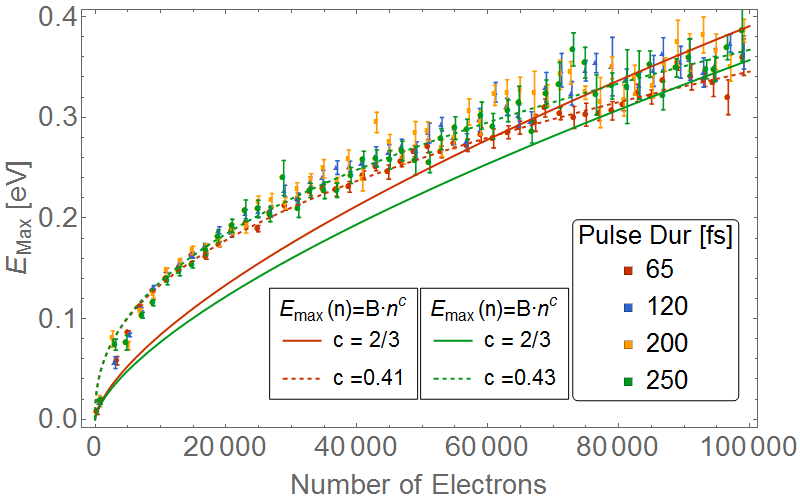
\includegraphics[width=8.4cm]{../Images/results/MIR_He_pulsescan/raw/binned.png}}
\hspace*{\fill}
\caption[MIR He pulse scan. Signal rate and Energy distribution]{On the left, Signal rate for the He-Xe  pulse duration scan. On the right, the binned energy distribution for the maximum Energy respect to the number of electrons. In colors are the different pulses and the errors bar is the standard derivation for the binned data every 1000 electrons and the dashes line are the fitted parameters.}
\label{fig:mult1}
\end{figure}

In fig \ref{Hepulsedur} we show the histograms as well as the Mean number of electrons and E$_{max}$  with dependency on the pulse duration. On top, the histograms shows a clear peak for the shorter duration while in the longest the distribution get broader. It means, that the smaller droplets are easily ignited on the shorter pulses, so we see the peak close to 100000 electrons, and on contrast, the longer pulses are more sensible to coulomb explode the bigger droplets. This also can be seen in the lower figures where the mean values rises with the pulse, in the energy and in the number of electrons. This result is surprising, especially if we compare it with Fig. \ref{fig:MIRwaterintenhisto}, in the Intensity dependence. 


\begin{figure}[htb]
\captionsetup[subfloat]{farskip=2pt,captionskip=1pt}
\centering
\hspace*{\fill}%
\subfloat{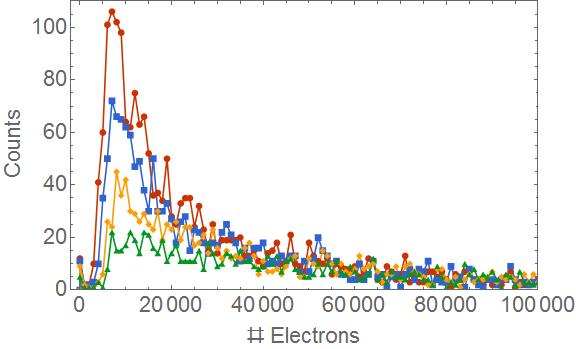
\includegraphics[width=0.4\textwidth]{../Images/results/MIR_He_pulsescan/raw/histoElec.png}}
\subfloat{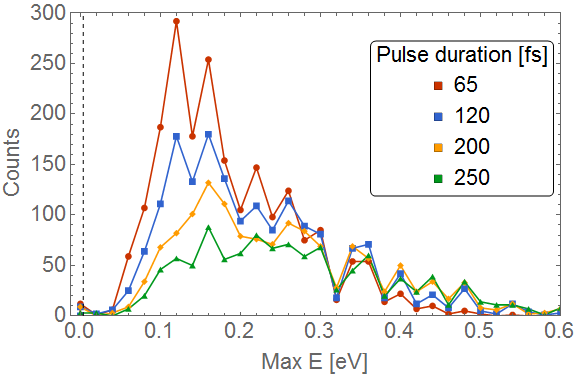
\includegraphics[width=7.5cm]{../Images/results/MIR_He_pulsescan/raw/histoEnergc.png}}
\hspace*{\fill}%
\subfloat{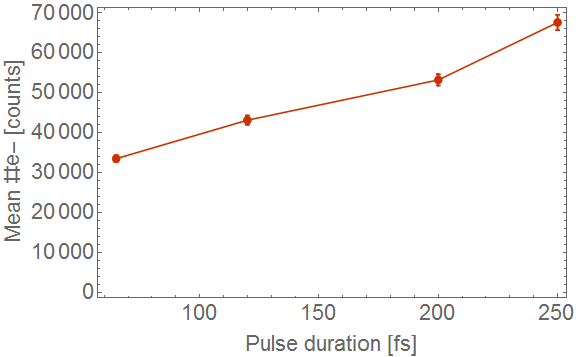
\includegraphics[width=0.4\textwidth]{../Images/results/MIR_He_pulsescan/raw/meanelect.png}}
\subfloat{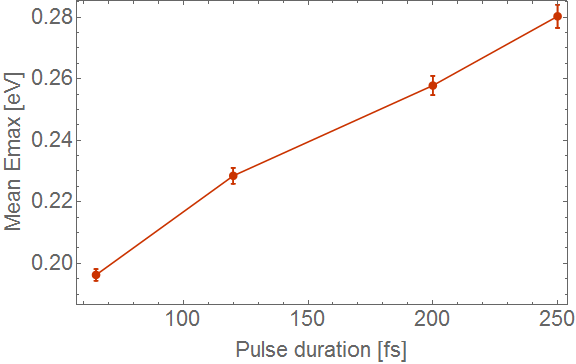
\includegraphics[width=0.4\textwidth]{../Images/results/MIR_He_pulsescan/raw/meanenergt.png}}
\hspace*{\fill}%
\caption[MIR He pulse scan. Mean values and Histograms]{On the top, Histograms for number of electro (left) and maximal energy (right) for the different pulses. On bottom, The mean $\#$e- and energy from the energy distribution for each pulses}
\label{Hepulsedur}
\end{figure}

As mentioned, the longer the pulse the weaker is its intensity. In fig \ref{Hepulsedur} we showed that the mean values in the Intensity scan decrease with the power in contrast to the pulse dependence where the mean values increases negligible the intensity. Although, it is a non-intuitive results, it can be explained if we take into account that for longer pulses we have more cycles in the pulse. In consequence, even the initial ionization probability is lower for the first cycles, the electrons created on them will have more time to interact with the laser field, acquiring more energy and incrementing the electronic cascade that will start the coulomb explosion.




\subsection{MIR. Helium-Xenon-Calcium doping scan}

In this experiment Helium clusters where doped with Xenon and Calcium atoms simultaneously. The Helium clusters were created at the same nozzle temperature $T_{nozzle}=10.6$ K and  a backing pressure of $P_{0}=30$ mbar. Xenon where introduce at 5 different pressures measured in the gas doping cell and Calcium was evaporated in the oven at 7 different temperatures. Table \ref{tab:dopXeCa} shows the sorted parameters used and their associate cluster size. The cells in the index (up and left) represent the number of atom for the Xenon and calcium for each data set while the inner cell shows their correlates mean He cluster size in atoms, The spaces in black are data set that were not taken.
The VMI voltages where set to VMIx1 and the MCP and PHS to $1600$V and $4000$V respectively. The camera was stablish to exposure time of $t_{exp}=34 \mu$s and single shot was ensure. The laser power where monitored constantly guarantee an average power of 10.7 W at pulses duration around $45$ fs.

\begin{table}[]
\label{tab:dopXeCa}
\centering
\begin{tabular}{|l|l|c|l|l|l|}
\hline
\backslashbox{Ca$_{dop}$}{Xe$_{dop}$} & \multicolumn{1}{c|}{0 atoms} & 30 & 90 & 180 & 350 \\ \hline
5 atoms & 241500 & 239100 & 234300 &  &  \\ \hline
7 & 239000 & \multicolumn{1}{l|}{236600} & 231800 &  &  \\ \hline
15 & 226300 & 223900 & 219100 &  &  \\ \hline
22 & 213400 & 211300 & 207080 &  &  \\ \hline
31 & 195500 &  & 189450 & 182550 & 172120 \\ \hline
45 & 170700 & \multicolumn{1}{l|}{} & 165150 & 159700 &  \\ \hline
62 & 137000 & \multicolumn{1}{l|}{} & 132050 & 127322 & <N>$_{He_{atoms}}$ \\ \hline
\end{tabular}
\end{table}

In Fig \ref{fig:HeXECAall} we present the binned energy distribution and its respective histograms for $\#$e- and E$_{max}$. All the different doping are plotted in the same diagram in order to show that the initial doping doesn't change radically the energy distribution. As usual, the points are the individual pictures bloop analyzed and binned, the dash lines are the fit for the corresponding Eq. 3.12 with variable factor founded on $2/5$ and a average B-factor of B$=0.0048$, leading to electronic cloud radii of $R=18 \mu$m. In this cases, we will not focus on the energy distribution because as shown, not big difference in the final electronic cloud is present. Further, the histograms we can show that the E$_{max}$ distribution is quite similar for all doping as well.  There is a defined peak close to 0.1 eV Boltzmann distribution likewise with a slow slop up to 0.4 eV. Furthermore, the number of electrons present a peak close to 2000 electrons with the slop decreasing up to 8000 where the counts reduce below 10. A second result to take into account, mentioned in the past chapters, is that the histogram share a peak electrons but the counts are reduce because of the signal rate as expected, so the dopant level does not play a big role in all state of the nanoplasma, But as we will see next, it does act in the signal rate and mean values.


\begin{figure}[htb]
\label{fig:HeXECAall}
\captionsetup[subfloat]{farskip=2pt,captionskip=1pt}
\centering
\hspace*{\fill}%
\subfloat{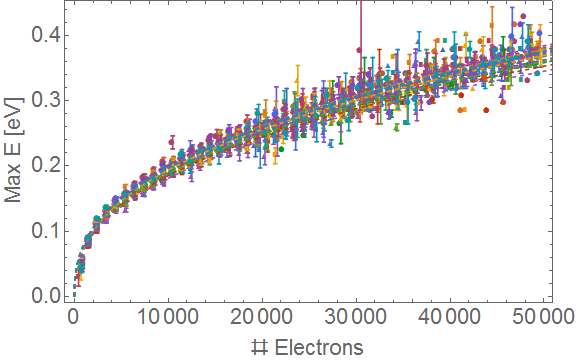
\includegraphics[width=0.33\textwidth]{../Images/results/MIR_He_XeCaDop/binned.png}} \subfloat{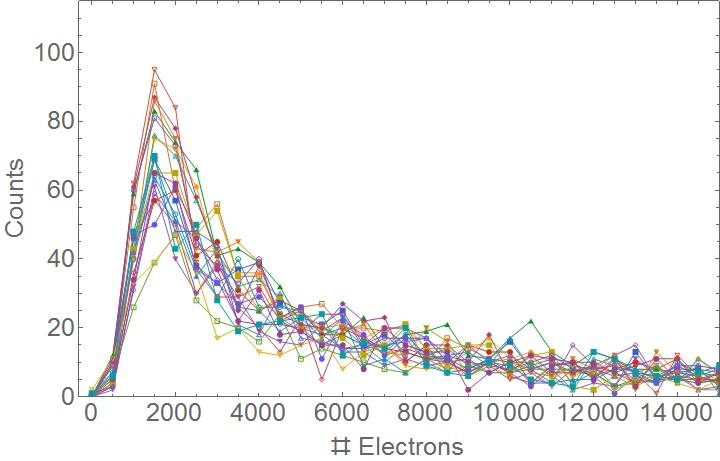
\includegraphics[width=0.3\textwidth]{../Images/results/MIR_He_XeCaDop/histoElectr.png}}\subfloat{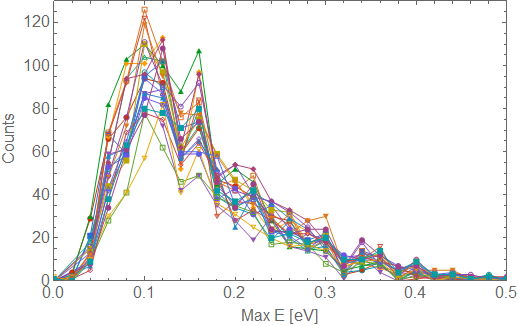
\includegraphics[width=0.3\textwidth]{../Images/results/MIR_He_XeCaDop/histoEnerg.png}
\hspace*{\fill}%
\caption[MIR He-Xe-Ca doping]{On The left, the binned energy distribution in function of the number of electrons for all the different doping levels in Xe and Ca, in color points the binned data and in dashed lines the corresponding fit function. In the center, the histogram for the Number of electrons for all doping levels. On the right, the histogram as well for the Max energies fount for all the doping. The doping have a joined behaviors, the counts derivate a few but is related to the signal rate as shown next. }
\end{figure}

Fig \ref{fig:HeXECA-signalrate} shows an interpolation for the signal rate. The green scale shows the percentage of signal in the data set for each doping level. On bottom the number of Xenon atoms and on left the number of calcium atoms. The white points represent the points where the measurement were done. The data points with higher dopant are also included in the interpolated but not plotted. The dashed color line are cuts at a constant dopant numbers, for different constant  Xe+Ca at $40,50,65,85,100,120$ and $150$ atoms. The lines where choose in order that each line lay between 3 data points, so the interpolation could be accurate enough. On the right of fig \ref{fig:HeXECA-signalrate}, the cuts are plotted depending on the Xe atoms. This means that the right side of each line represent the doping with the maximum Xe atoms at the Xe+Ca constant,  once we go from right to left, we replace each Xe atom for one  Ca atom until we replace all Xe atom. Each line have a maximum of 40 points, because it was the max Ca doping measured. 


An important result can de derive from Fig \ref{fig:HeXECA-signalrate}, as shown in the cut lines at constant total doping, we found a increment in the signal as the Ca doping replace the Xe. In all line, from right to left, the signal rate goes up when a few atoms of Ca are added despite the amount of Xe. It demonstrate a better efficiency in the doping for Xe-Ca combination compared to only Xe or only Ca. This tendency can be spot not just on the big crest in the interpolation between 70 to 120 Xe atoms and 15 to 25 Ca atoms, but also in each of the cuts, where the peaks are clearly display and the signal rate increase faster for these extra Ca atoms added, but once we reach a saturation maxima, the extra Ca atoms added makes the signal rate again decrees but in a slower way in most of the cases. 

\begin{figure}[htb]

\captionsetup[subfloat]{farskip=2pt,captionskip=1pt}
\centering
\hspace*{\fill}%
\subfloat{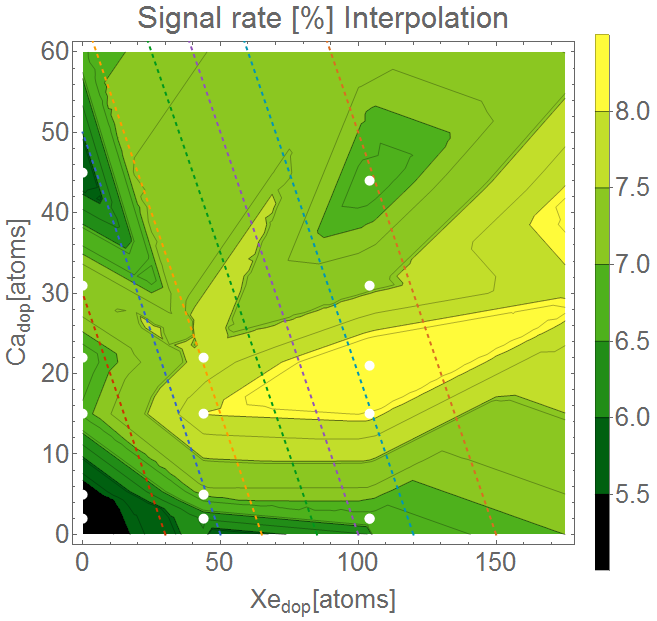
\includegraphics[width=0.4\textwidth]{../Images/results/MIR_He_XeCaDop/interpolationSignalRate.png}}\hfill  \subfloat{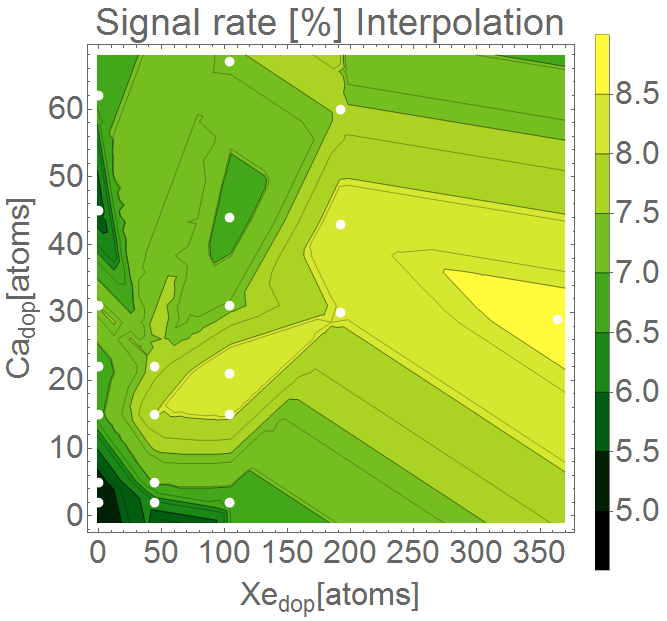
\includegraphics[width=0.48\textwidth]{../Images/results/MIR_He_XeCaDop/interpolationSignalRate2.png}
\hspace*{\fill}%
\caption[MIR He-Xe-Ca doping Signal rate]{Interpolation and Cuts for the Signal Rates at different. The Green graph is the interpolation of all the different doping levels with Xe and Ca. On white points, the actual measurements and in dashes colored lines, the cuts at constant doping level. On the right, the plot of signal rate depending on Xe doping for the corresponding cuts at the same color.}
\label{fig:HeXECA-signalrate}
\end{figure}


The same interpolation  was done for the histograms for the  number of electrons and maximum energy, Fig \ref{fig:HeXECA-NUmEle} and Fig. \ref{fig:HeXECA-Emax} shows the interpolation and cuts for constant dopant respectively. Fig \ref{fig:HeXECA-NUmEle} show one clear peak at low doping where the maximum  number of electrons appears, then for higher doping the counts starts to decreases and even a small depletion is shown in the range of Xe=100 Ca=20 atoms. On the right, the cut at constant dopant is show, the color from left to right represent the same cut done in the corresponding interpolation, and it’s necessary to read it at the same way. Where the right side of each line represents just Xe doping and each number to the left mean replacing one Xe atom for one Ca atom. As show, the exist also a recurrent peak efficiency in the nanoplasma ignition, meaning that at this peak the larger cluster are ionized, similar as shown on the Pulse duration scan. 



\begin{figure}[htb]

\captionsetup[subfloat]{farskip=2pt,captionskip=1pt}
\centering
\hspace*{\fill}%
\subfloat{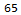
\includegraphics[width=0.4\textwidth]{../Images/results/MIR_He_XeCaDop/interpolationE.png}}\hfill  \subfloat{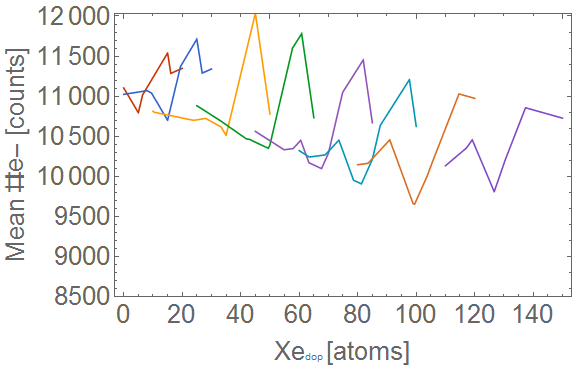
\includegraphics[width=0.48\textwidth]{../Images/results/MIR_He_XeCaDop/interpolationE2.png}
\hspace*{\fill}%
\caption[MIR He-Xe-Ca doping Mean Num Electrons]{ Interpolation and Cuts for the Mean values at different doping of the number of electrons.  The Green graph is the interpolation of all the different doping with Xe and Ca. On white points, the actual measurements and in dashes colored lines, the cuts at constant doping level. On the right, the plot on Xe doping dependence for the cut with the same color.}
\label{fig:HeXECA-NUmEle}
\end{figure}

Equally important. In the E$_{max}$ interpolation, a clear peak is also shown at Xe= 50 and Ca=7 atom, where the highest energy is present and a slow drop start for  heavier doping. At larger number of dopant the interpolation is less effective due the lack of measurement, so for smaller droplets at heavy doping the cluster starts to deform and deplete it so the nanoplasma explosion is not possible. This can be found in interpolation cuts, where the highly doped lines have a more constant performance and no real change is shown, but once we get close to the optimum doping (Yellow line), the replacement of Xe atom for Ca atoms becomes drastic effective, with a peak  founded close to 0.2 eV.  This measurement can be compare directly to the water doping scan where we show that once the ignition of the cluster starts, adding more water atoms does not creates changes in the process. Here, Xe doping results in a similar behavior, the points with just Xe atoms (Right edge of each colored line) have a relative constant mean energy, but once we introduce the Ca, dynamics start to appears, given a peak close to the Mean electrons interpolation. For the heavily doped clusters, on the blue, orange and purple cuts in the right, we see that the peaks are not present any more due the cluster destruction when to many atoms are added.

\begin{figure}[htb]
\label{fig:HeXECA-Emax}
\captionsetup[subfloat]{farskip=2pt,captionskip=1pt}
\centering
\hspace*{\fill}%
\subfloat{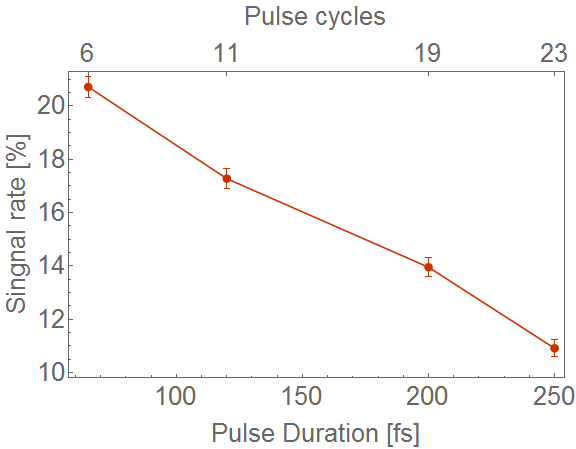
\includegraphics[width=0.4\textwidth]{../Images/results/MIR_He_XeCaDop/interpolationMax.png}}\hfill  \subfloat{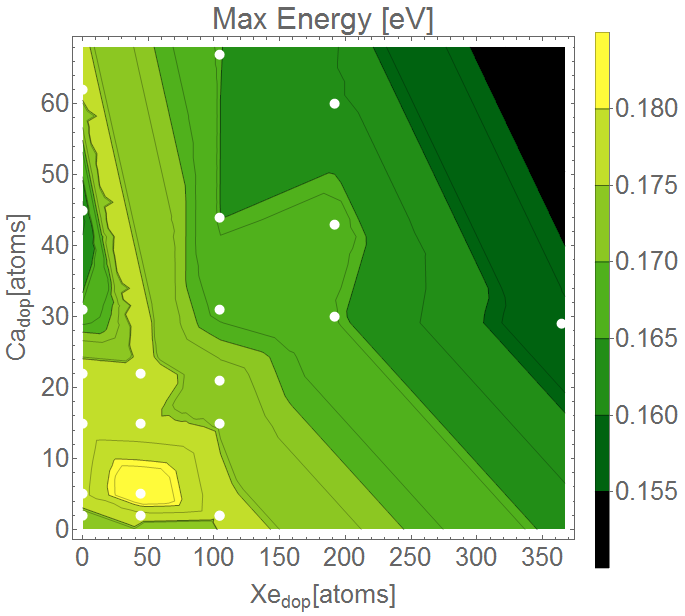
\includegraphics[width=0.48\textwidth]{../Images/results/MIR_He_XeCaDop/interpolationMax2.png}
\hspace*{\fill}%
\caption[MIR He-Xe-Ca doping Mean Max energy]{Interpolation and Cuts for the Mean values at different doping for the Maximum energy measured. The Green graph is the interpolation of all the different doping with Xe and Ca. On white points, the actual measurements and in dashes colored lines, the cuts at constant doping level. On the right, the plot on Xe doping 	 for the cut with the same color.}
\end{figure}


If we compare the three interpolation, in a similar way we have analyzed the histogram in the last sections, we notice that the signal rate have a peak close to Xe=100 and Ca=20, but the Mean number of electrons and energy appears at lower doping. This means that at the most efficient rate, we are not igniting the biggest droplets but on contrary, they are being exploded closer to the zero doping.


\section{Neon nanoplasma under Mid-Infrared}

In the next section we present the results for the second beam time at ELI-Alps where we examines the nanoplasma formation for Neon clusters under Mid-Infrared laser pulses. The laser for this experiment was the same system used in Helium droplets. Neon cluster were created via a supersonic expansion with a conical nozzle with aperture d=15 $\mu$m of diameter. In order to obtain different cluster sizes, we used several nozzle temperatures around 37 K to 42 K, with a constant backing pressure of 50 mbar. Neon 0.6 XXX were used to assure the purity of the clusters and to avoid any nozzle clog. Neon was doped with Xenon through the gas doping cell. We will present 3 different experiments; Neon clusters size, Laser Pulse duration scan and Xe doping dependence. The VMI voltages keeps the same rate and the MCP and PHS voltages will be specified in each section. The pressures in the detection chamber oscillated during the experiments around 6E-8 mbar with the chopper open (Cluster beam in).  

Neon cluster formation presents a technical challenge due its solidification curve, at this backing pressure, small changes on the nozzle temperature leads to solidification of the gas, so we need to be careful at temperatures lower than 37 K. Another difference between Neon and Helium, is that the Neon clusters after the supersonic expansion are in a solid state. Same as performed with the Helium cluster, we use the Hagena scale to estimate the cluster sizes. Despite the difference and changes in the parameters, we perform the experiments without further problems.

\begin{figure}[h!]
\centering
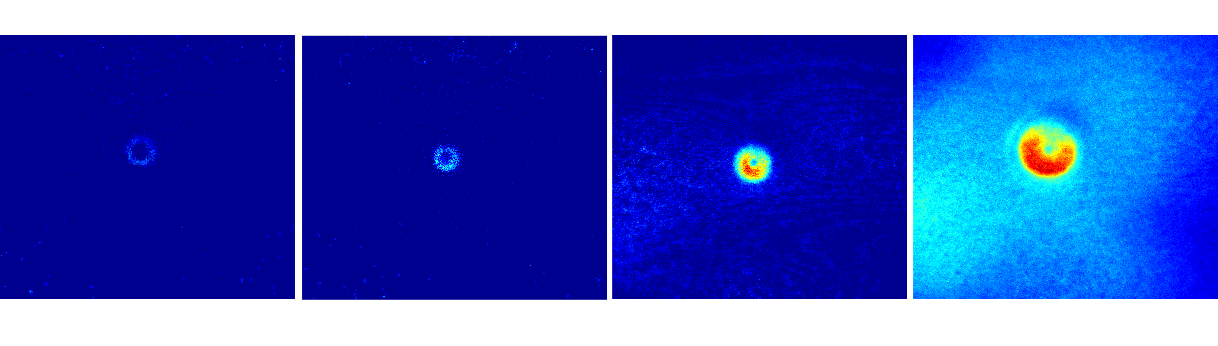
\includegraphics[width=1\textwidth]{../Images/Raw MIR NEon samples.png}
\caption[MIR Neon raw samples]{Sample signals for the Neon nanoplasma. }
\label{fig:neonrwasample}
\end{figure}

Fig \ref{fig:neonrwasample} show a compilation of the raw VMI signals of Neon plasma. In general all pictures have a similar distributions to the helium clusters. Fig. a and b are the most common signals, with very small bloops and weak intensity, specially at temperatures upper than 39 K.  Fig \ref{fig:neonrwasample} c represent a small rate of the images upper 39 K, where the bloops get bigger and higher intensities are present. The anisotropic  brightness  in the two last samples, are due a blind spot in the upper-center of the phosphorscreen developed because the large amount of signals collected during the days. Fortunately it is a systematic error and for future experiments we will just need to replace the detector. Additionally Fig  \ref{fig:neonrwasample} d are the signals for biggest droplets  at 37 K, the bloops start to be anisotropic and saturating the camera. Although, this signals was not a significant percentage of the results, they did appear regularly. One explanation for its irregular outline is given if we assume big clusters with irregular shapes, because the Neon clusters are solid, the bigger clusters will not condensate uniformly and in consequence they will create anomalies on the signal. Another explanation could be because of the large density of electron in big nanoplasma, they start to interact and create an unusual signal. Subsequently, this big droplets will be analyzed independently. 

\subsection{MIR. Neon-Xenon doping scan}

In this experiment Small Neon clusters where doped with Xenon at different doping levels. The Neon clusters were created at the same nozzle temperature $T_{nozzle}=39$ K and at a backing pressure of $P_{0}=50$ mbar. Xenon where introduce at 7 different pressures measured in the oven chamber. The VMI voltages were set to VMIx1 and the MCP and PHS to $1700$ V and $4000$ V respectively. The camera was stablish to an exposure time of $t_{exp}=34$ $\mu$s  and the laser power were set to an average power of 10 W.


\begin{figure}[h!]
\centering

\hspace*{\fill}
{ 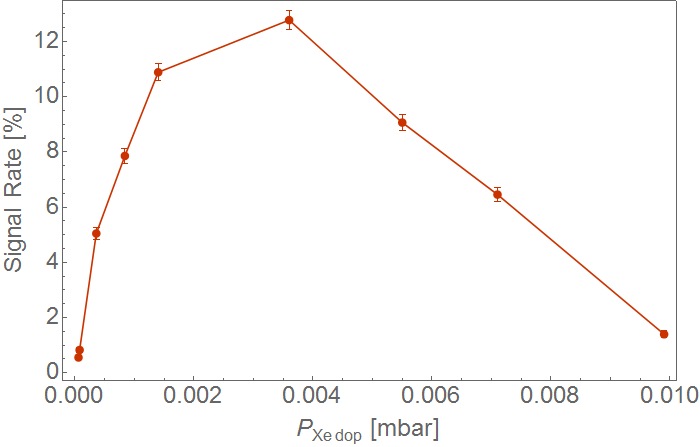
\includegraphics[width=6cm]{../Images/results/MIR_Ne_XeDop_39K/SigRate.png}} \hfill {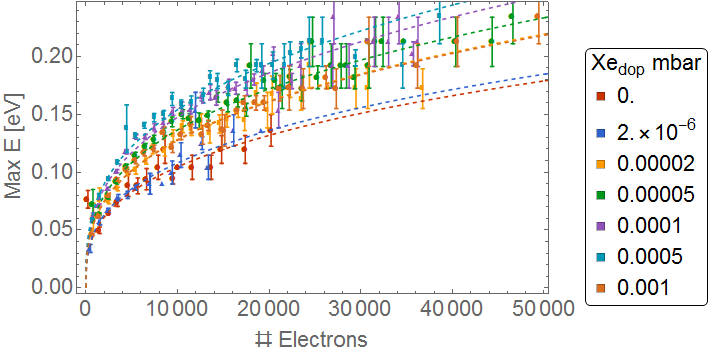
\includegraphics[width=7.4cm]{../Images/results/MIR_Ne_XeDop_39K/binned.png}}
\hspace*{\fill}
\caption[MIR Ne-Xe doping scan. Signal rate and Energy distribution]{On the left, Signal rate for the Ne-Xe doping scan. On the right, the binned energy distribution for the maximum Energy respect to the number of electrons. In colors are the different doping pressures and the errors bar is the standard derivation for the binned data every 1000 electrons and the dashes line are the fitted parameters.}
\label{fig:NeonsigrateXedop}
\end{figure}


Fig \ref{fig:NeonsigrateXedop}, shows the signal rate for the different pressures and the energy distribution for all doping levels. As notice on the left of the plot, the nanoplasma signal rate increase rapidly with the doping, until the best doping at 5E-5 mbar and keep constant for higher doping. This agrees to our previous results showing there exist a minimum doping level to have the most efficient plasma creation, and stronger doping does not help to have more signal. On contrary, for the highest doping levels we denote a small reduction in the signal rate showing that at this level, the clusters starts to be destroyed, and the signal rate goes down.
For the Energy distribution, each colored point is the binning of the individual signal transformed to number of electrons and Energy, the dashed lines are the fits to the data according Eq 3.13 with $k$ and $B$ factor set free. As seen in the plot, the fit functions are quite similar to each other, sharing a comparable distribution. Table XXX shows the exponent, B-factor and the corresponding density and radius for the electronic cloud found from the fit. This functions agrees perfectly to or spherical cloud model, same as it happened on the NIR experiments. This relation proof that the Islam Model applied to the electron in a nanoplasma explosion could be accurate.

\begin{figure}[htb]
\captionsetup[subfloat]{farskip=2pt,captionskip=1pt}
\centering
\hspace*{\fill}%
\subfloat{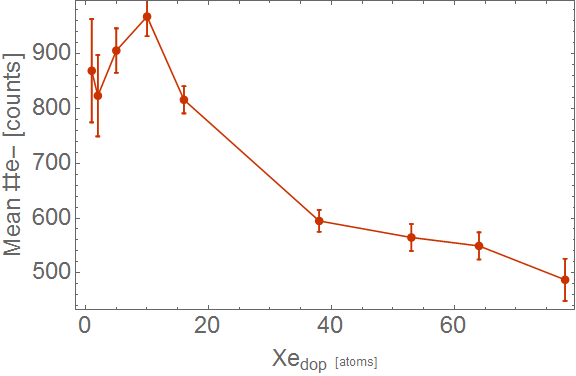
\includegraphics[width=0.35\textwidth]{../Images/results/MIR_Ne_XeDop_39K/MeanEnerg.png}
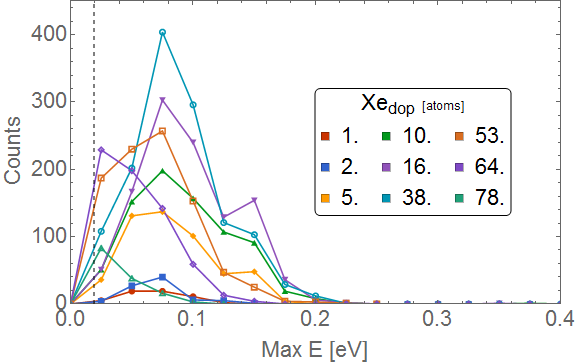
\includegraphics[width=0.4\textwidth]{../Images/results/MIR_Ne_XeDop_39K/HEnergc.png}}
\hspace*{\fill}%

\hspace*{\fill}%
\subfloat{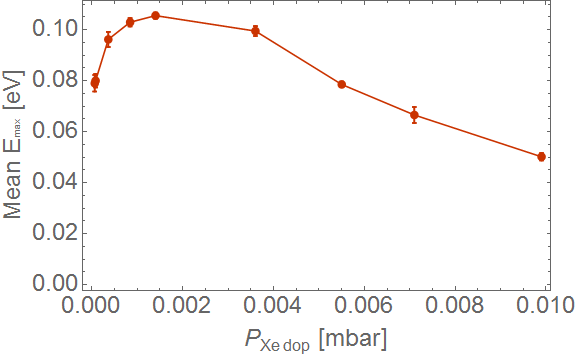
\includegraphics[width=0.35\textwidth]{../Images/results/MIR_Ne_XeDop_39K/MeanElec.png}
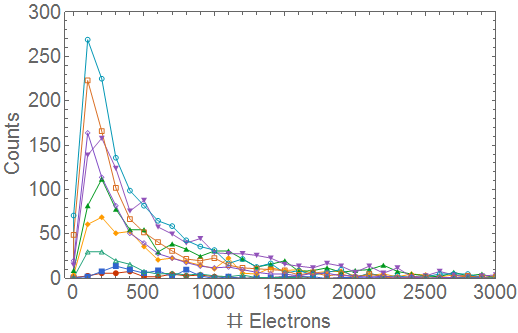
\includegraphics[width=0.4\textwidth]{../Images/results/MIR_Ne_XeDop_39K/HElec.png}}
\hspace*{\fill}%
\caption[MIR Neon Doping scan. Mean values and Histograms]{On the top, Histograms for number of electro (left) and maximal energy (right) for the different Xenon doping levels. On bottom, the mean $\#$e- and energy from the energy distribution for each pressure}
\label{fig:NehistoDoping}
\end{figure}



Fig. \ref{fig:NehistoDoping} shows the histogram and the mean values for the Max energy and number of electrons. On the top, the histogram show a close distribution with peaks close to 0.1 eV and a drastic decrease up to 0.2 eV, showing as well, the recurrent off value in the min energy required by the plasma that is close to zero but no zero. On the electrons histogram, a broader distribution is shown with a systematic peak at 3000 electrons, it means that the mean signal found, correspond to small clusters, even though  massive signals up to 30000 electrons can be found. On one hand, The mean values shows a constant increment in the energy for the first pressures, going in agreement with the signal rate, in other words, adding more dopant to the  Neon allows to achieve higher energies, but after reaching the doping limit pressure, a decrease in the mean energy appears. On the other hand, for the mean number of electrons, we see that for the first doping, the mean value keeps quite constants, but once we go upper the 5E-5 mbar, the mean decrease but the signal rate keeps high. This results shows that the doping increase the efficiency to ignite the nanoplasma, but at large doping level the mean value of electrons decrease, meaning that we are igniting small droplets. In short, is more efficient to ignite bigger droplets than small ones, because according to the data, the small ones need a larger amount of doping to be ignited while the large cluster just need a few atoms.

\subsection{MIR. Neon cluster size scan}

In order to understand the nano plasma explosion in Neon cluster, this experiment was done on different Neon cluster at a fix doping level with Xenon. The Neon clusters were created at 5 nozzle temperature 39, 40, 41, 42 and 44 K with a backing pressure of $P_{0}=50$ mbar. Xenon where introduce at a fix  pressures measured in the doping cell of 0.00036 mbar. The VMI voltages  where set to VMIx1  and the MCP and PHS to $1800$ V and $4100$ V respectively. The camera was stablish to exposure time of $t_{exp}=34$ $\mu$s   with the single shoot measurement scheme. The laser power were set to an average power of 11 W.

\begin{figure}[htb]
\centering

\hspace*{\fill}
{ \includegraphics[width=6cm]{../Images/results/MIR_Ne_DropletSize/SigRate.png}} \hfill {\includegraphics[width=7.4cm]{../Images/results/MIR_Ne_DropletSize/binned.png}}
\hspace*{\fill}
\caption[MIR Ne-Xe cluster Size scan. Signal rate and Energy distribution]{On the left, Signal rate for neon at different nozzle temperatures. On the right, the binned energy distribution for the maximum Energy respect to the number of electrons. In colors are the different doping pressures and the errors bar is the standard derivation for the binned data every 1000 electrons and the dashes line are the fitted parameters.}
\label{fig:NeonsigrateDropltesize}
\end{figure}

Fig \ref{fig:NeonsigrateDropltesize} shows the signal rate and the energy distribution for the different nozzle temperatures. On the left, the signal rate shows an expected result where the bigger droplets present the higher rates and it decrease with the cluster size (high temperatures). We can compare this result with Fig. \ref{fig:NIRsrEnergy} where it have the same behaviour. The reason for this tendency is not clear, but if we assume the interaction dopant-cluster, small cluster could have a high probability of losing the ionized electrons in the beginning of the pulse, so the ignition process is less efficient, while for the bigger clusters, the ionized electron have more atoms to interact, so the losses are less, and in consequence the bigger clusters are more efficient to create the nanoplasma. For the Energy distribution there is no surprise neither, the data point and signal presents the same energy distribution as shown in the doping scan, The fit function was once again done based on Eq. 3.13 and give a exponent of $2/3$ following the spherical model. For the B factor, was in average $B=0.09$ given a density of 62 $\mu$m$^{-3}$ and a electronic cloud radius of 7 $\mu$m.

\begin{figure}[h!]
\captionsetup[subfloat]{farskip=2pt,captionskip=1pt}
\centering
\hspace*{\fill}%
\subfloat{\includegraphics[width=0.35\textwidth]{../Images/results/MIR_Ne_DropletSize/MeanEnerg.png}
\includegraphics[width=0.4\textwidth]{../Images/results/MIR_Ne_DropletSize/HEnergc.png}}
\hspace*{\fill}%

\hspace*{\fill}%
\subfloat{\includegraphics[width=0.35\textwidth]{../Images/results/MIR_Ne_DropletSize/MeanElec.png}
\includegraphics[width=0.4\textwidth]{../Images/results/MIR_Ne_DropletSize/HElec.png}}
\hspace*{\fill}%
\caption[MIR Neon Size scan. Mean values and Histograms]{On the top, Histograms for number of electro (left) and maximal energy (right) for the different Neon nozzle temperatures. On bottom, The mean $\#$e- and energy from the energy distribution for each pressure}
\label{fig:Nehistosize}
\end{figure}


The mean values show in Fig. \ref{fig:Nehistosize} also have a trivial behaviour, congruent to the signal rate, both, mean number of electrons and Max energy, show a decrease with the cluster size. This trend is also present in Fig. \ref{fig:NIR2}, but for smaller droplets. The Histogram on the right, have a clear broaden distribution and it have a smaller off set in the zero again. The energy count present a peak around 0.05 eV and almost none signal is present over 2 eV. Furthermore, The number of electrons have a similar trend  with a peak around 3000 electrons, analogous to the histogram in the Xe doping scan.

\subsection{MIR. Neon pulse scan}

The last measurement done in Eli Alps- was a laser pulse duration scan. Neon cluster at a fix doping level with Xenon at a  nozzle temperature 39 K and a backing pressure of $P_{0}=50$ mbar  were shoot by the MIR laser pulse at 5 different pulse duration of, 48, 55, 64 71, and 94 fs. Xenon where introduce at a fix pressures measured in the doping cell at 0.0002 mbar. The VMI voltages were set to VMIx1 and the MCP and PHS to $1700$ V and $4000$ V respectively. The camera was stablish to exposure time of 34 $\mu$s with the single shoot measurement scheme. As in section 4.2.5 the pulse duration have a recurrent effect in the laser power, Table \ref{tab:Neonpulsepower} shows the different powers and consecutive the laser intensities at each data set was taken, as shown all sets are comparable.

\begin{table}[t]
\centering

\begin{tabular}{|l|l|c|}
\hline
Pulse duration {[}fs{]} & \multicolumn{1}{c|}{Power{[}W{]}} & Laser intensity {[}W/Cm$^{2}${]} \\ \hline
48 & 10.5 & 2E14 \\ \hline
55 & 11 & 1.7E14 \\ \hline
64 & 11 & 1.5E14 \\ \hline
71 & 10.4 & 1.3E14 \\ \hline
94 & 8.6 & 1E14 \\ \hline
\end{tabular}
\caption{Neon pulse scan  intensity table.}
\label{tab:Neonpulsepower}
\end{table}


\begin{figure}[htb]
\centering

\hspace*{\fill}
{ \includegraphics[width=6cm]{../Images/results/MIR_Ne_pulseduration/SigRate.png}} \hfill {\includegraphics[width=7.4cm]{../Images/results/MIR_Ne_pulseduration/binned.png}}
\hspace*{\fill}
\caption[MIR Ne Pulse duration scan. Signal rate and Energy distribution]{On the left, Signal rate for neon at different pulse duration. On the right, the binned energy distribution for the maximum Energy respect to the number of electrons. In colors are the different doping pressures and the errors bar is the standard derivation for the binned data every 1000 electrons and the dashes line are the fitted parameters.}
\label{fig:Neonsigratepulse}
\end{figure}


Fig. \ref{fig:Neonsigratepulse} present the signal rate and the energy distribution for the different pulse duration. Here the signal rates shows the same tendency that sec 4.2, The pulse duration plays an important role in the nanoplasma ignition, and the probability to create nanoplasma decrease constantly with the pulse, in this case, almost having no signal for pulses longer than 100 fs. The Energy distribution on the other hand, also shows a similitude to the helium results, The Max energy and number of electrons keep a mark distribution around the fit function, the dashed lines correspond to the fit function with a exponent of 2/3 and a B- factor of 0.0004.





\begin{figure}[h!]
\captionsetup[subfloat]{farskip=2pt,captionskip=1pt}
\centering
\begin{subfigure}[l]{1\textwidth}
\includegraphics[width=0.49\textwidth]{../Images/results/MIR_Ne_pulseduration/MeanEnerg.png}
\includegraphics[width=0.49\textwidth]{../Images/results/MIR_Ne_pulseduration/HEnerg.png}  				\end{subfigure}
\centering
\begin{subfigure}[l]{1\textwidth}
\includegraphics[width=0.49\textwidth]{../Images/results/MIR_Ne_pulseduration/MeanElec.png}
\includegraphics[width=0.49\textwidth]{../Images/results/MIR_Ne_pulseduration/HElec.png} 				\end{subfigure}
\caption[MIR Neon pulse duration. Mean values and Histograms]{MIR Neon pulse duration. On the top, mean values (Left) and Histogram (right) for the max energy. At the Bottom mean values (Left) and Histogram (right) for the number of electrons at different pulse duration.}
\label{fig:Nehistopulse}
\end{figure}




Surprisingly in Fig \ref{fig:Nehistopulse} the mean values for the electron numbers and energy also shown a strong relation to the pulse duration. As table \ref{tab:Neonpulsepower} reefers, the intensity that the laser gave were almost the same, so the variations in the mean values confirm that at longer pulses the rates to ionize bigger droplets increase. So as shown, we can see the same effect regardless the cluster element and doping level. For understand this result we need to picture how the stretch of a pulse will derive in more cycles in it. The first cycles will be determinant for the Ionization of the dopant, the electrons create in the beginning of the pulse will have more time to interact with the laser field, and in consequence they will acquire more energy and time to interact with the cluster. Once we stretch the pulse, the electrons produced in this first cycle will see more cycles, and the ionization of the cluster will be more efficient. 






